\documentclass[12pt]{article}
\usepackage{braket}
\usepackage{physics}
\usepackage{simplewick}
\usepackage{relsize}
\usepackage{graphicx}
\usepackage{times}
\usepackage[export]{adjustbox}
\usepackage{listings}
\usepackage{mathcomp}
\usepackage{hyperref}
\usepackage{bm,amsmath}
\usepackage{amssymb}
\usepackage{float}
\usepackage{indentfirst}
\usepackage{bigints}
\usepackage{listings}
\usepackage{color}
\usepackage{cite}
\usepackage{slashed}
\usepackage{amsmath}
\hypersetup{
colorlinks=true,
linkcolor=blue,
filecolor=magenta,
urlcolor=cyan,
pdftitle={Overleaf Example},
pdfpagemode=FullScreen,
}
\definecolor{dkgreen}{rgb}{0,0.6,0}
\definecolor{gray}{rgb}{0.5,0.5,0.5}
\definecolor{mauve}{rgb}{0.58,0,0.82}
\lstset{frame=tb,
language=Python,
aboveskip=3mm,
belowskip=3mm,
stepnumber = 1,
showstringspaces=false,
columns=flexible,
basicstyle={\small\ttfamily},
numbers=left,
numberstyle=\color{gray},
keywordstyle=\color{blue},
commentstyle=\color{dkgreen},
stringstyle=\color{mauve},
breaklines=true,
breakatwhitespace=true,
tabsize=3
}
\numberwithin{equation}{section}
\makeindex

\newcommand\be{\begin{eqnarray}}
\newcommand\ee{\end{eqnarray}}
\newcommand\f\phi
\newcommand\cO{\mathcal{O}}
\newcommand\p[1]{\left(#1\right)}
\newcommand\ptl\partial
\newcommand\e\epsilon
\newcommand\<\langle
\renewcommand\>\rangle
\newcommand\Z{\mathbb{Z}}
\newcommand\de\delta
\newcommand\R{\mathbb{R}}
\newcommand\bx{\mathbf{x}}
\newcommand\nn{\nonumber}
\renewcommand\.{\cdot}
\newcommand\x\times
\newcommand\pdr[2]{\frac{\partial #1}{\partial #2}}
\newcommand\s\sigma
\newcommand\SO{\mathrm{SO}}
\newcommand\De{\Delta}
\newcommand\cS{\mathcal{S}}
\newcommand\oo\infty
\newcommand\SU{\mathrm{SU}}
\newcommand\cH{\mathcal{H}}
\newcommand\bn{\mathbf{n}}
\newcommand\bP{\mathbf{P}}
\renewcommand\b\beta
\renewcommand\a\alpha
% \newcommand\Tr{\mathrm{Tr}}
\renewcommand\l\lambda
\newcommand\cL{\mathcal{L}}
\newcommand\cD{\mathcal{D}}
\renewcommand\th{\theta}
\newcommand\tl[1]{\widetilde{#1}}

\title{QFTII Final Project\\Conformal Bootstrap}
\author{Ting-kai Hsu}
\date{\today}

\begin{document}
\maketitle
\tableofcontents
\begin{abstract}
    
\end{abstract}
\section{Introduction to Conformal Bootstrap and Its Language}

This section encompasses the first three chapters of Simmons-Duffin's TASI lecture notes \cite{simmonsduffin2016tasilecturesconformalbootstrap}, where we provide a brief overview of the bootstrapping philosophy, along with the foundational language and conventions used in this field.

\subsection{Bootstrap Philosophy}
The critical universality of many microscopic theories allows us to focus on the CFT.

\subsection{Path Integral Quantization}
Path integral formalism chooses a specific time direction, and spacetime is divided into successive slices. Each slice is associated with a Hilbert space of states in the Heisenberg picture, and the progression from one slice to the next is governed by time evolution. The general correlator is defined as follows:

\begin{equation}
    \langle\mathcal{O}_1(x_1)\cdots\mathcal{O}_n(x_n)\rangle = \bra{0}\text{T}\left\{\hat{\mathcal{O}_1}(t_1,\mathbf{x}_1)\cdots\hat{\mathcal{O}_n}(t_n,\mathbf{x}_n)\right\}\ket{0}
\end{equation}

Here, note that the L.H.S represents a product of spacetime functions. At the same time, the R.H.S. is a product of operators in the Heisenberg picture, defined in distinct Hilbert spaces corresponding to each slice. This is the familiar form of the correlator within the path integral framework.

\subsection{Stress Energy and Topological Surface Operator}
Consider a quantum field theory (QFT) coupled to a background metric $g$,  with correlators defined within the path integral formalism in Euclidean signature. 
\begin{equation}
    \bra{0}\text{T}\left\{\hat{\mathcal{O}_1}(t_1,\mathbf{x}_1)\cdots\hat{\mathcal{O}_n}(t_n,\mathbf{x}_n)\right\}\ket{0}_{g} = \int{\prod_{y}d\phi(y)\,\mathcal{O}_1(x_1)\cdots\mathcal{O}_n(x_n)e^{-S[g,\phi]}}
\end{equation}
The stress-energy tensor is the conserved current associated with the diffeomorphism invariance of the action $S[g,\phi]$ in the flat spacetime limit $g\rightarrow\eta$.
% \begin{equation}
%     \langle T^{\mu\nu}(x)\mathcal{O}_1(x_1)\cdots\mathcal{O}_n(x_n)\rangle_g = \frac{2}{\sqrt{|g(x)|}}\frac{\delta}{\delta g_{\mu\nu}(x)}\langle\mathcal{O}_1(x_1)\cdots\mathcal{O}_n(x_n)\rangle_{g}
% \end{equation}
% Around the flat spacetime limit, we derive the familiar Ward-Takahashi identity\footnote{See appendix.}:
Consequently, we obtain the familiar Ward-Takahashi identity:
\begin{equation}
    \partial_{\mu}\langle T^{\mu\nu}(x)\mathcal{O}_1(x_1)\cdots\mathcal{O}_n(x_n)\rangle = -\sum_{i}\delta^4(x-x_i)\partial^{\nu}_{i}\langle\mathcal{O}_1(x_1)\cdots\mathcal{O}_n(x_n)\rangle
\end{equation}

Define \textbf{topological surface operator}:
\begin{equation}
    P^{\nu}(\Sigma)\equiv-\int_{\Sigma}{dS_{\mu}}T^{\mu\nu}(x)
\end{equation}
The integral is taken over a closed hypersurface within the spacetime manifold, which can be considered the boundary of a ball $B$. The presence of delta functions in the Ward-Takahashi identity allows for the deformation of this closed hypersurface, provided that the deformation does not intersect additional spacetime points. Let's consider a ball $B$ that encloses a spacetime point $x$ where an operator $\mathcal{O}(x)$ insertion occurs. In this case, the volume integral over the ball transforms into a surface integral over the boundary of $B$ on the L.H.S:
\begin{equation}
\begin{split}
    \langle P^{\nu}(\Sigma)\mathcal{O}(x)\cdots\rangle = \int_{B}{d^4y\delta^4(y-x)}\partial^{\nu}_{x}\langle\mathcal{O}(x)\cdots\rangle\\
    =\partial^{\nu}\langle\mathcal{O}(x)\cdots\rangle
\end{split}
\end{equation}

\begin{figure}[h]
\centering
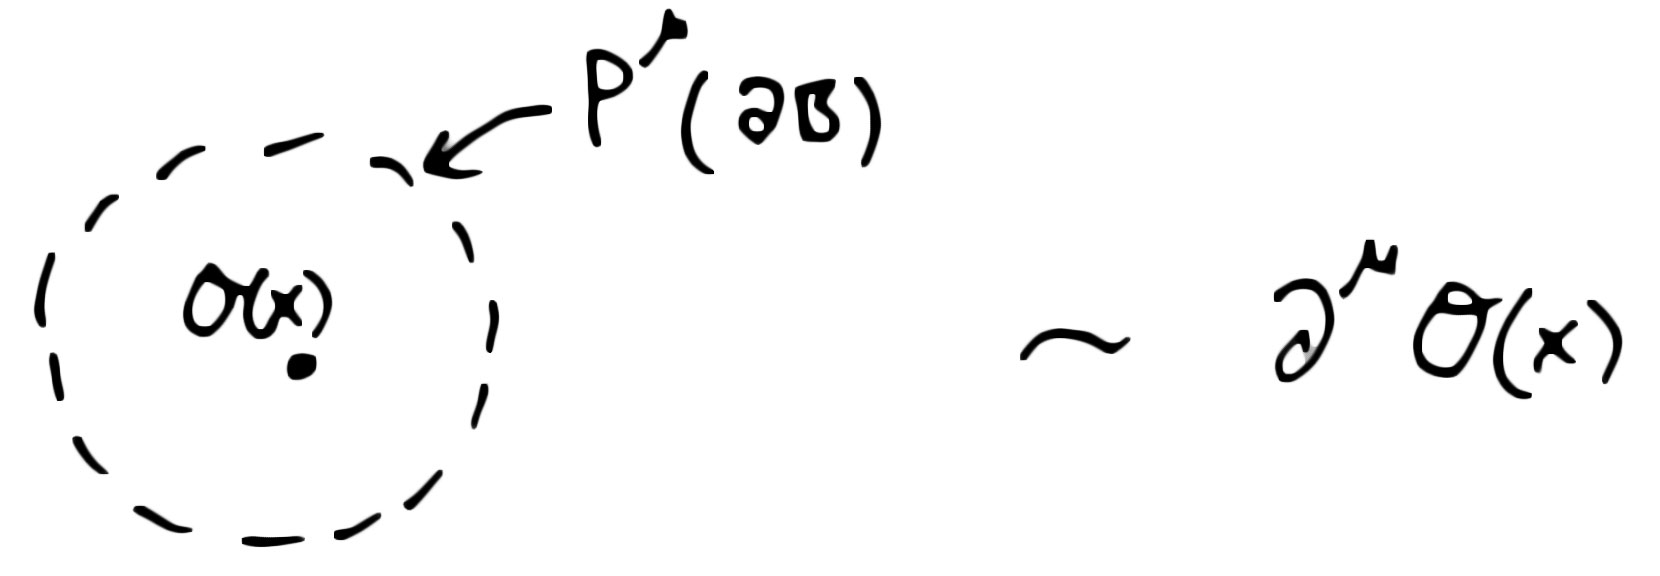
\includegraphics[width=0.5\textwidth]{surroundoperator.jpg} % Placeholder for Fig.1
\caption{\label{surroundoperator}Illustration of the topological operator loop.}
\end{figure}

\indent As long as no additional spacetime points with operator insertions are crossed, the surface \( \Sigma \) can be freely deformed from one slice to another, maintaining the invariance of \( P^{\mu}(\Sigma) \). This invariance implies that the momentum \( P^{\mu}(\Sigma) \) is topological in the path integral formulation, which in turn indicates that it is conserved.
Now, consider two spatial slices at times \( t_1 \) and \( t_2 \) within the spacetime manifold, with \( t_1 < t_2 \). Suppose there is an operator insertion \( \mathcal{O}(t, \mathbf{x}) \) at a time \( t \) such that \( t_1 < t < t_2 \). If we "sandwich" this operator between the slices at \( t_1 \) and \( t_2 \), then:

\begin{equation}
    \lim_{t_1\rightarrow t_2^{-}}\langle P^{\mu}(\Sigma_2)\mathcal{O}(x)\cdots\rangle-\langle P^{\mu}(\Sigma_1)\mathcal{O}(x)\cdots\rangle = \bra{0}\text{T}\left\{\left[\hat{P}^\mu,\hat{\mathcal{O}}(x)\right]\cdots\right\}\ket{0}
\end{equation}
The appearance of the commutator on the R.H.S arises due to the time ordering in the correlation function. Since the momentum \( P^{\mu}(\Sigma) \) is topological, we can deform \( \Sigma_2 - \Sigma_1 \) to a sphere \( S \) that encloses the local point \( x \):
\[
    \lim_{t_1\rightarrow t_2^{-}}\langle P^{\mu}(\Sigma_2)\mathcal{O}(x)\cdots\rangle-\langle P^{\mu}(\Sigma_1)\mathcal{O}(x)\cdots\rangle = \langle P^{\mu}(S)\mathcal{O}(x)\cdots\rangle 
\]
\[
    =\partial_{x}^{\mu}\langle\mathcal{O}(x)\cdots\rangle
\]
\begin{figure}[h]
\centering
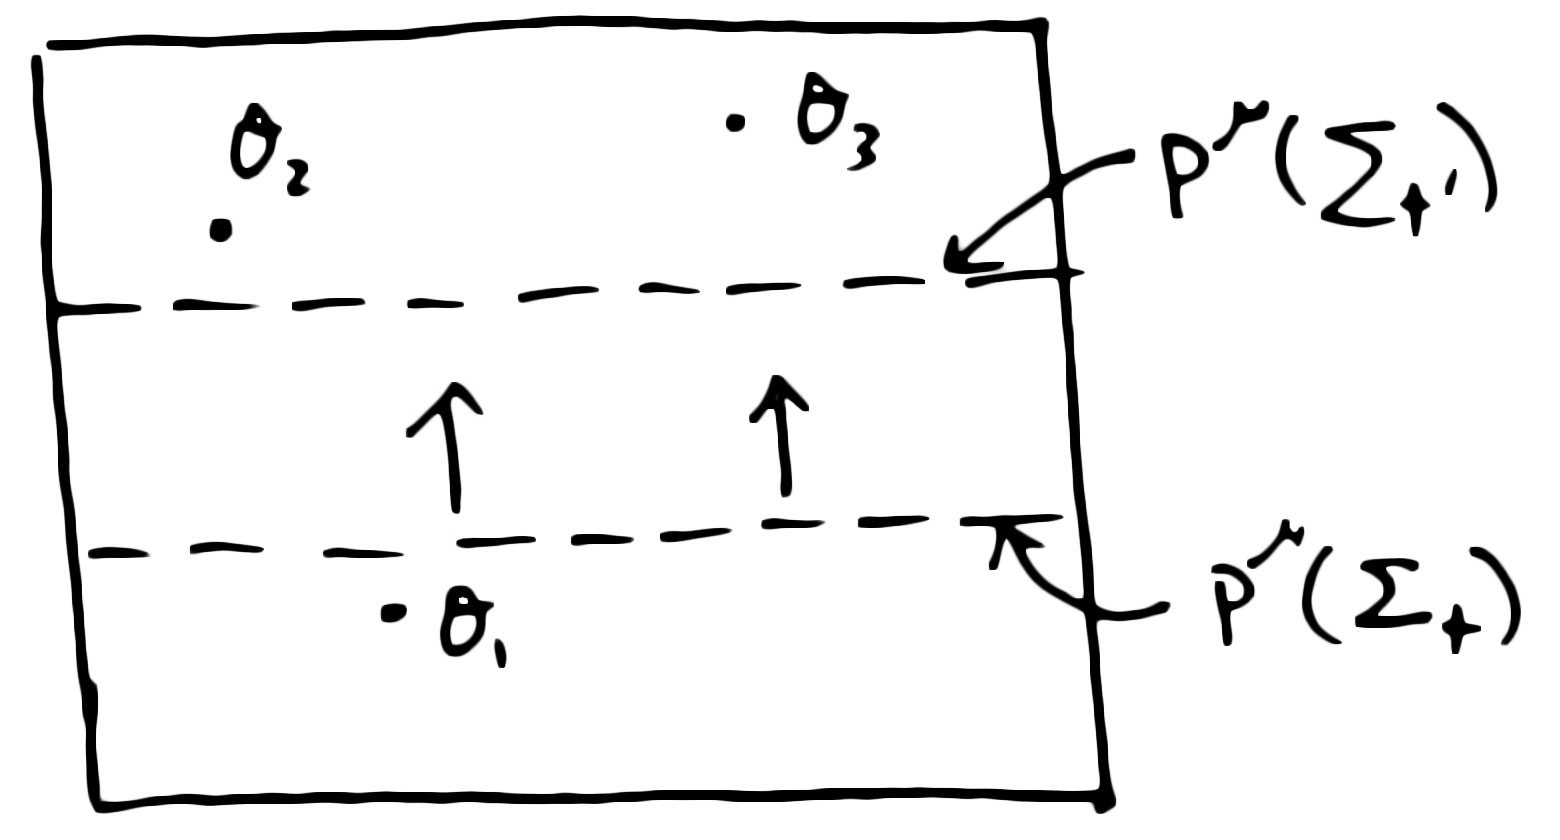
\includegraphics[width=0.5\textwidth]{slidingcharges.jpg} % Placeholder for Fig.2
\caption{\label{fig:slidingcharges} Illustration of the shrinking region in path integrals.}
\end{figure}
This is the familiar commutation relation for the momentum operator in quantum mechanics:
\begin{equation}
    \left[\hat{P}^{\mu}, \hat{\mathcal{O}}(x)\right] = \partial^{\mu}\hat{\mathcal{O}}(x)
\end{equation}
At first glance, the L.H.S of Eq(1.7) appears non-local because the topological momentum operator is expressed as a surface integral over a finite spacetime volume. However, by progressively deforming the boundary \( \Sigma \) to increasingly concentrate around the enclosed singularity, we reveal the locality of the transformation, as shown on the R.H.S of Eq(1.7).
\subsection{Conformal Symmetry}
Next, we can consider more symmetries, especially symmetries of general coordinate transform, infinitesimally,
\begin{equation}
    x^{\mu}\rightarrow x'^{\mu} = x^{\mu} + \epsilon^{\nu}(x)
\end{equation}
the corresponding conserved charge\footnote{One might argue why local symmetry can have a conserved charge, however, here we should view them as a special case.} as an infinitesimal transformation generator:
\begin{equation}
    Q_{\epsilon}(\Sigma) = -\int_{\Sigma}{dS_{\mu}\,}\epsilon_{\nu}(x)T^{\mu\nu}(x)
\end{equation}
Stress energy $T^{\mu\nu}(x)$ is assumed to be conserved, symmetry, and \textit{traceless}\footnote{Tracelessness of stress energy is related to conformal symmetry, as we're about to show.}, then the conservation of $Q$ implies:
\[
    \partial_{\mu}(\epsilon_{\nu}T^{\mu\nu}(x)) = 0
\]
\[
    =\frac{1}{2}\left(\partial_{\mu}\epsilon_{\nu}(x)+\partial_{\nu}\epsilon_{\mu}(x)\right)\cdot T^{\mu\nu}(x)
\]
Then, traceless $T^{\mu\nu}(x)$ leads to conformal Killing equation:
\begin{equation}
    \partial_{\mu}\epsilon_{\nu}(x) + \partial_{\nu}\epsilon_{\mu}(x) = \eta_{\mu\nu}c(x)
\end{equation}
Constant spacetime translation satisfies the equation and the corresponding conserved charge $Q_{\epsilon}$ is momentum, and we'll discuss more symmetries that are solutions to the conformal Killing equation in the appendix. In terms of $\epsilon(x)$, $c(x) = 2/d\,\partial\cdot\epsilon(x)$. To see how metric transforms, first consider,
\[
    \frac{\partial x'^{\mu}}{\partial x^{\nu}} = \delta^{\mu}_{\nu} + \partial_{\nu}\epsilon^{\mu}(x)
\]
\begin{equation}
    \approx \left(1+\frac{c(x)}{2}\right)\left(\delta^{\mu}_{\nu} + \frac{1}{2}(\partial_{\nu}\epsilon^{\mu}-\partial^{\mu}\epsilon_{\nu})\right)
\end{equation}
where we've used conformal Killing equation and ignore $\mathcal{O}(\epsilon^2)$ terms. The R.H.S of Eq(1.11) is an infinitesimal rescaling times an infinitesimal rotation. Equivalently, the transformation $x\rightarrow x'$ governed by the conformal Killing equation and stress energy rescales the metric by a scalar factor. Such transformations are called \textit{conformal}\footnote{By conformal, we mean the angles between two curves' intersections are invariant under the transformations, as can be seen from the transformation of metric.}.
% \subsection{More on Topological Surface Operator}
First, let’s build our language about operators and states through the path integral and prepare some materials needed later. From our course, we’ve learned that
\begin{equation}
\label{eq1}
\ldots
\end{equation}

If we contact $O$ with other operators, then we get
\begin{equation}
\label{eq2}
\ldots
\end{equation}

We could use the path integral to prove \eqref{eq2}, which will be left in the appendix.

Then, consider the integral of $J$ over a closed surface:
\begin{equation}
\label{eq3}
\ldots
\end{equation}

From \eqref{eq2} and the divergence theorem, we can find a correlator of $J$ is only related to what operators appear in its loop, instead of the path itself (shown in Fig.~1). $J$ is called the “topological (codimension-1) operator.” If we act $J$ onto other operators, it is equivalent to taking the derivative, as:
\begin{equation}
\label{eq4}
\ldots
\end{equation}

In this language, the topological codimension-1 operator is the same as having a symmetry.

Also, from our course last semester, we’ve known the correlation function could be written as:
\begin{equation}
\label{eq5}
\ldots
\end{equation}

Then, we can do two different path integrals $Z$ concerning $J$. The integral should be time-ordered, so by subtracting each other, it will shrink into a region surrounding (shown in Fig.~2). Then by \eqref{eq4}, we could get its commutation relation:
\begin{equation}
\label{eq6}
\ldots
\end{equation}



Integrating \eqref{eq6} over $J$, we will get:
\begin{equation}
\label{eq7}
\ldots
\end{equation}
which shows how we represent the operator away from the origin with the one at the origin.
\section{Conformal Algebra}

The conformal symmetry of spacetime is expressed by an extension of the Poincaré group, known as the conformal group. Conformal symmetry encompasses special conformal transformations and dilations and has 15 degrees of freedom in $3+1$ dimensions.



The Lie algebra of the conformal group has the following representation:
\be
\label{eq:angularmomentum}
M_{\mu\nu} \equiv x_{\mu}\ptl_{\nu}-x_{\nu}\ptl_{\mu}
\ee
\be
\label{eq:momentum}
P_{\mu}\equiv \ptl_{\mu}
\ee
\be
\label{eq:dilatation}
D\equiv x_{\mu}\partial_{\mu}
\ee
\be
\label{eq:specialconformaltransformation}
K_{\mu} = 2x_{\mu}(x^{\nu}\ptl_{\nu})-x^2\ptl_{\mu}
\ee

Where $M_{\mu\nu}$ are the Lorentz generators, $P_\mu$ generates translations, which are also the generators in the Poincaré group. Also, $D$ generates scaling transformations (also known as dilatations or dilations) and $K_\mu$ generates the special conformal transformations. It can be shown that these generators can be determined by the traceless stress tensor $T^{\mu\nu}$. A more rigorous discussion about conformal symmetry, conformal transformation, and how to solve its killing equations will be left in the appendix.

From the definition of generators (\ref{eq:angularmomentum})-(\ref{eq:specialconformaltransformation}), we can then derive their commutation relations, as (\ref{eq:angularmomentummomentumcmr})-(10), and all other commutators are zero.

\be
\label{eq:angularmomentummomentumcmr}
\begin{split}
[M_{\mu\nu}, P_\rho] &= [(x_\mu \partial_\nu - x_\nu \partial_\mu), \partial_\rho] \\
&= [x_\mu \partial_\nu, \partial_\rho] - [x_\nu \partial_\mu, \partial_\rho] 
\\
&= -\delta_\rho^\mu P_\nu + \delta_\rho^\nu P_\mu.
\end{split}
\ee

\be
\label{eq:angmomSCTcmr}
\begin{split}
[M_{\mu\nu}, K_\rho] &= [(x_\mu \partial_\nu - x_\nu \partial_\mu), 2x_\rho (x^\sigma \partial_\sigma) - x^2 \partial_\rho] \\
&= 2\big(x_\mu \delta_{\nu\rho} x^\sigma \partial_\sigma - x_\nu \delta_{\mu\rho} x^\sigma \partial_\sigma\big) 
+ \big(x^2 \delta_{\rho\mu} \partial_\nu - x^2 \delta_{\rho\nu} \partial_\mu\big) \\
&= \delta_{\nu\rho}\big(2x_\mu (x \cdot \partial) - x^2 \partial_\mu\big) 
- \delta_{\mu\rho}\big(2x_\nu (x \cdot \partial) - x^2 \partial_\nu\big) \\
&= \delta_{\nu\rho} K_\mu - \delta_{\mu\rho} K_\nu.
\end{split}
\ee

\[
(7) \quad \ldots
\]
\[
(8) \quad \ldots
\]
\[
(9) \quad \ldots
\]
\[
(10) \quad \ldots
\]



Note that (5)-(7) show that $P_\mu$ and $K_\mu$ transform as vectors under rotation $SO(d)$ and $J_{\mu\nu}$ generates this algebra. (8)-(10) illustrate that $P_\mu$ and $K_\mu$ are lowering and raising operators of $D$, which is similar to $SU(2)$ algebra introduced in the quantum mechanics course.

Formally, we can define $X^M$, where the index $M$ runs from $-1$ to the dimension $d+1$. If we define $X^M$ in the way (11)-(15), then $J_{MN}$ will satisfy the commutation relations of $SO(d+1,1)$:
\[
(11) \quad \ldots
\]
\[
(12) \quad \ldots
\]
\[
(13) \quad \ldots
\]
\[
(14) \quad \ldots
\]

Therefore, it is better to treat the algebra in space $\mathbb{R}^{d+1,1}$ than $\mathbb{R}^{d,1}$, which is the idea of embedding space formalism. In this formalism, we would define another vector $X^M$ in $\mathbb{R}^{d+1,1}$, compared to $x^\mu$ in $\mathbb{R}^{d,1}$, and $X^M$ should have restrictions:
\[
(15) \quad \ldots
\]
\[
(16) \quad \ldots
\]

Since (15)-(16) give two restrictions to $X^M$, roughly speaking, the space described by $X^M$ has the same dimension as $\mathbb{R}^{d,1}$, and $x^\mu$ are “embedded” in $X^M$.


\section{Primary Operator and Correlation Function}
\section{Radial Quantization and Cylindrical Quantization}
\section{Operator Product Expansion}

Two operator products $\cO_i(x)\cO_j(0)$ can be covered inside a spacetime ball $B$ that can separate them from other operator insertions. Every state on the boundary $\partial B$ can be decomposed as a linear combination of primaries and descendants, then
\be
\label{eq:opeinitial}
\cO_i(x)\cO_j(0)|0\> &=& \sum_{k}C_{ijk}(x,\hat{P})\cO_k(0) |0\>,
\ee
where $k$ runs over primary operators and $C_{ijk}(x, \hat{P})$ is an operator, which becomes a coefficient depending on primary operators as the position is taken to be closed to origin $x\rightarrow 0$.

\begin{figure}[h]
\begin{center}
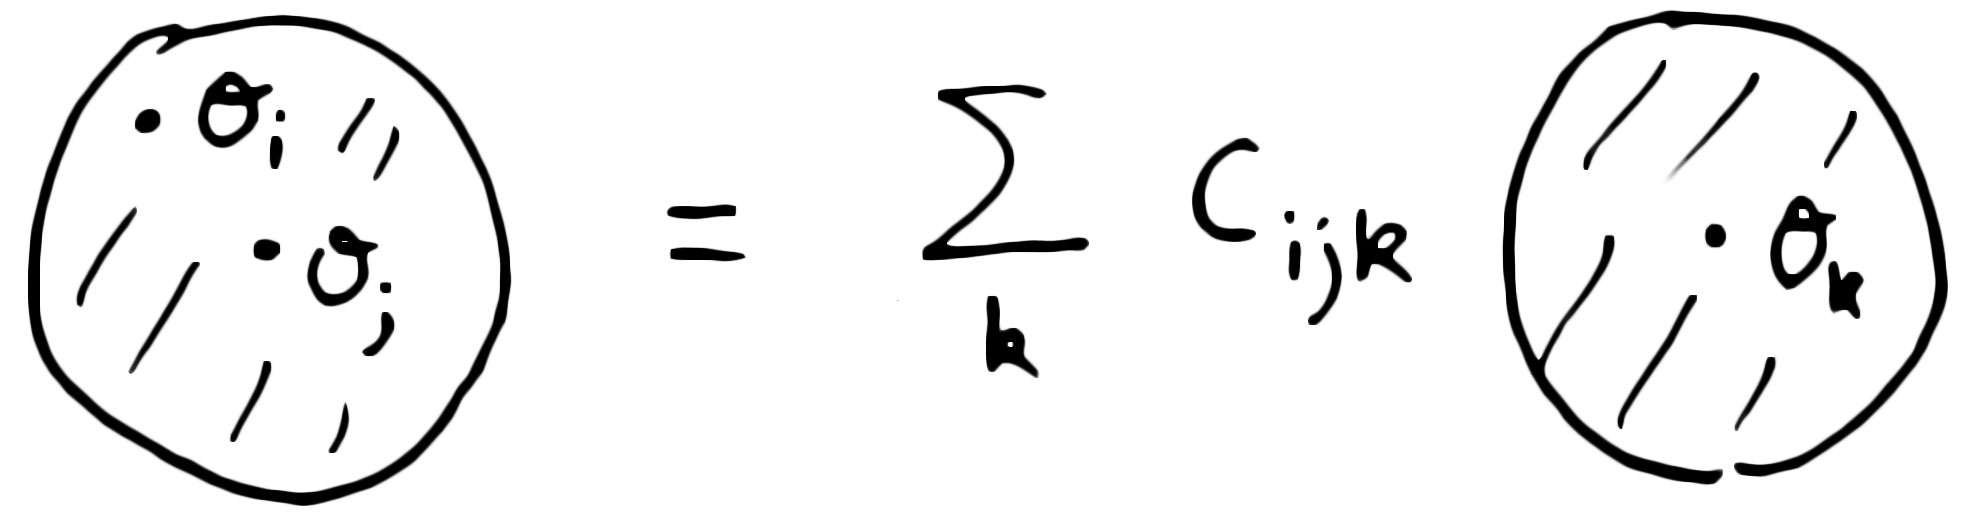
\includegraphics[width=0.6\textwidth]{ope.jpg}
\end{center}
\caption{A state created by two operator insertions can be expanded as a sum of primary states with position-dependent coefficient.  
\label{fig:ope}}
\end{figure}

Using the state-operator correspondence and promoting the momentum operator $\hat{P}\rightarrow\partial$
\be
\label{eq:opeinitial2}
\cO_i(x_1)\cO_j(x_2) &=& \sum_{k}C_{ijk}(x_{12},\ptl_2)\cO_k(x_2),\qquad\textrm{(OPE)}
\ee
where it is understood that (\ref{eq:opeinitial2}) is valid inside any n-point correlation function where the other operator insertions $\cO_n(x_n)$ far away from them, $|x_{2n}| \geq |x_{12}|$. Eq.~(\ref{eq:opeinitial2}) is called the Operator Product Expansion (OPE). Operator product expansion can be thought of as an analog to Taylor expansion in calculus, and extract the divergence of infinite fluctuation due to small separation into coefficients, with the remaining part represented by a single operator.

We could alternatively perform an expansion around a different point $x_3$ that a sphere centered at $x_3$ encloses $x_1$ and $x_2$, giving
\be
\label{eq:opealternative}
\cO_i(x_1)\cO_j(x_2) &=& \sum_k C'_{ijk}(x_{13},x_{23},\ptl_3)\cO_k(x_3),
\ee
where $C'_{ijk}(x_{13},x_{23},\ptl_3)$ is some other differential operator (figure~\ref{fig:radialquantotherpoint}). (\ref{eq:opealternative}) shows that we can do the OPE whenever it's possible to draw any sphere that separates the two operators from all the other operator insertions in spacetime.

\begin{figure}[h]
\begin{center}
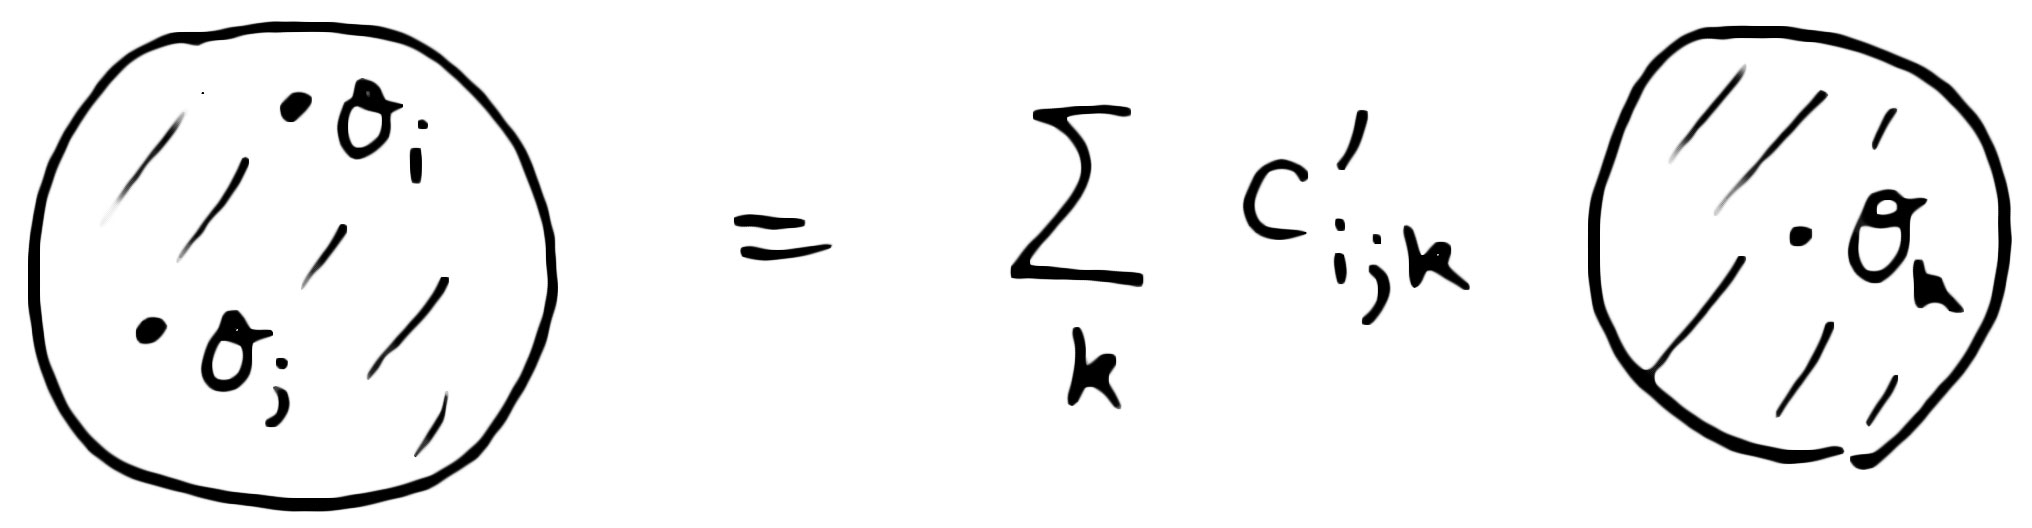
\includegraphics[width=0.6\textwidth]{radialquantotherpoint.jpg}
\end{center}
\caption{OPE doesn't have to be centered at the origin, and the expansion basis is located at some spacetime point as the dependence 
 of the other operator's position is absorbed by the coefficients. \label{fig:radialquantotherpoint}}
\end{figure}

If the primaries carry spins, the OPE then becomes
\be
\cO_i^a(x_1)\cO_j^b(x_2) &=& \sum_k C_{ijk}^{AB}{}_c(x_{12},\ptl_2)\cO_k^c(x_2),
\ee
where $a,b,c$ are indices for (possibly different) representations of $\SO(d)$.

% \noindent\rule[0.5ex]{\linewidth}{1pt}
By acting on both sides of (\ref{eq:opeinitial}) with $D$,
\[
\begin{split}
\text{RHS} = 
\left(D\cO_i(x)\right)\cO_j(0)|0\> - \left(\cO_i(x)D\right)\cO_j(0)|0\> + \cO_i(x)\left(D\cO_j(0)\right)|0\>
\\
-\cO_i(x)\left(\cO_j(0)D\right)|0\> + \cO_i(x)\cO_j(0)|0\>
\\
= \left[D,e^{iP\cdot x}\cO_{i}(0)\right]\cO_j(0)|0\>+\Delta_{j}\cO_i(x)\cO_j(0)|0\> + \cO_i(x)\cO_j(0)|0\>
\end{split}
\]

\[
\begin{split}
\text{LHS} = 
\sum_{k}DC_{ijk}(x,\hat{P})\cO_{k}(0)|0\> - \sum_{k}C_{ijk}(x,\hat{P})D\cO_{k}(0)|0\>
\\
+ \sum_{k}C_{ijk}(x,\hat{P})D\cO_{k}(0)|0\>
\\
= \sum_{k}\left[D,C_{ijk}(x,\hat{P})\right]\cO_{k}(0)|0\> + \sum_{k}\Delta_{k}C_{ijk}(x,\hat{P})\cO_{k}(0)|0\>+\cO_{i}(x)\cO_{j}(0)|0\>
\end{split}
\]
Then we have a differential equation of coefficient,
\be
\label{eq:differentialcoefficient}
\begin{split}
\left[D,C_{ijk}(x,\hat{P})\right] = 
\\
(\Delta_i+\Delta_j-\Delta_k)C_{ijk}(x,\hat{P}) + x^{\mu}\cdot\ptl_{\mu} C_{ijk}(x,\hat{P})
\end{split}
\ee

The solution is given in order by order $\cO(x\cdot \hat P)$
\be
\label{eq:opeexpansionexample}
C_{ijk}(x,\ptl) &\propto& |x|^{\De_k-\De_i-\De_j}\p{1 + C_1 x^\mu\ptl_\mu + C_2 (x\cdot\ptl)^2+ C_3 x^2 \ptl^2 + \dots}\nn\\
\ee
% \noindent\rule[0.5ex]{\linewidth}{1pt}

\subsection{Consistency with Conformal Invariance}
% \begin{exercise}
% \end{exercise}
By conformal invariance, such as dimensional analysis, rotational invariance, and non-trivially, and the special conformal transform, the form of the coefficient in OPE is strongly restricted.

We get a more interesting constraint by acting with SCT $K_\mu$, for simplicity, suppose $\cO_i$, $\cO_j$, and $\cO_k$ are scalars. Consistency with $K_\mu$ completely fixes $C_{ijk}$ up to an overall coefficient so that the coefficients of each term in (\ref{eq:opeexpansionexample}) are determined.

Take the correlation function of both sides of (\ref{eq:opeinitial2}) with a third operator $\cO_k(x_3)$ (Assume $|x_{23}|\geq |x_{12}|$, so that the OPE of $\cO_i(x_1)\text{ and }\cO_j(x_2)$ is valid),
\be
\label{eq:threetotwo}
\<\cO_i(x_1)\cO_j(x_2)\cO_k(x_3)\> &=& \sum_{k'} C_{ijk'}(x_{12},\ptl_2)\<\cO_{k'}(x_2)\cO_k(x_3)\>.
\ee

The three-point function on the left-hand side is fixed by conformal invariance, as mentioned in the previous sections. Choosing \textbf{an orthonormal basis of primary operators} for the expansion, so that $\<\cO_{k'}(x_2)\cO_{k}(x_3)\>= \de_{kk'}x_{23}^{-2\De_k}$.  The sum then collapses to a single term, giving
\be
\label{eq:matchingthreept}
\frac{f_{ijk}}{x_{12}^{\De_i+\De_j-\De_k}x_{23}^{\De_j+\De_k-\De_i}x_{31}^{\De_k+\De_i-\De_j}} &=& C_{ijk}(x_{12},\ptl_2)x_{23}^{-2\De_k}.
\ee
This determines that $C_{ijk}$ is proportional to $f_{ijk}$, times a differential operator that depends only on $\De_i$' s. The coefficient operator can be obtained by matching both sides of (\ref{eq:matchingthreept}) in small expansion $|x_{12}|/|x_{23}|$.
% \begin{exercise}
% \label{exercise:seriesfordiffops}

% \noindent\rule[0.5ex]{\linewidth}{1pt}
If $\De_i=\De_j=\De_\f$, and $\De_k=\De$, then (\ref{eq:opeexpansionexample}) becomes
\be
\label{eq:identicalscalaropeoperator}
C_{ijk}(x,\ptl) &=& f_{ijk} x^{\De-2\De_\f}\p{1+\frac 1 2 x\.\ptl + \a x^\mu x^\nu\ptl_\mu\ptl_\nu + \b x^2 \ptl^2+\cdots}\nn\\
\ee
% where
% \be
% \label{eq:opedescendantcoefficients}
% \a &=& \frac{\De+2}{8(\De+1)},\quad\textrm{and}\quad \b=-\frac{\De}{16(\De-\frac{d-2}{2})(\De+1)}.
% \ee

% \noindent\rule[0.5ex]{\linewidth}{1pt}
% \end{exercise}

\subsection{Correlation Function with OPE}

Equation (\ref{eq:threetotwo}) gives an example of using the OPE to reduce a three-point function to a sum of two-point functions.  In general, we can use the OPE to reduce any $n$-point function to a sum of $n-1$-point functions by the assumption of locality,
\be
\<\cO_1(x_1)\cO_2(x_2)\cdots\cO_n(x_n)\> &=& \sum_k C_{12k}(x_{12},\ptl_2)\<\cO_k(x_2)\cdots\cO_n(x_n)\>.\nn\\
\ee
Recursing, we can reduce everything to a sum of one-point functions, which are fixed by dimensional analysis,
\be
\<\cO(x)\> &=& \begin{cases}
1 & \textrm{if $\cO$ is the unit operator,}\\
0 & \textrm{otherwise.}
\end{cases}
\ee
This gives an algorithm for computing any flat-space correlation function using the OPE\@.  It shows that all these correlation functions are determined by dimensions $\De_i$ and three-point correlation function coefficients $f_{ijk}$.
% \footnote{The OPE is also valid on any conformally flat manifold.  The difference is that on nontrivial manifolds, non-unit operators can have nonzero one-point functions.  An example is $\R^{d-1}\x S^1_\b$, which has the interpretation as a CFT at finite temperature.  By dimensional analysis, we have $\<\cO\>_{\R^{d-1}\x S^1_\b}\propto \b^{-\De_\cO}\propto T^{\De_\cO}$.\label{foot:finitetemperature}}

\section{Conformal Blocks}

\subsection{Using the OPE}

We can use the OPE to compute a four-point correlation function of identical scalars. Recall that conformal invariance fixes the function up to some arbitrary function that is conformal-invariant
\be
\<\f(x_1)\f(x_2)\f(x_3)\f(x_4)\> &=& \frac{g(u, v)}{x_{12}^{2\De_\f}x_{34}^{2\De_\f}},
\ee
where the cross-ratios $u$, $v$ are given previous section.

On the other hand, the OPE of two scalar fields takes the form
\be
\label{eq:scalarscalarOPE}
\f(x_1)\f(x_2) &=& \sum_\cO f_{\f\f\cO} C(x_{12},\ptl_2)\cO(x_2),
\ee
% where $\cO^{a}$ can have nonzero spin in general. 
% For $\cO^a$ to appear in the OPE of two scalars, it must transform in a spin-$\ell$ traceless symmetric tensor representation of $\SO(d)$.
% \begin{exercise}

% Prove this as follows. Show that $\<\cO^a|\f(x)|\f\>$ vanishes unless $\cO^a$ is a symmetric tensor.  (Tracelessness comes from restricting to irreducible representations of $\SO(d)$.) Argue that if $\<\cO^a|\f(x)|\f\>$ vanishes, then for any descendant $|\psi\>=P\cdots P|\cO\>$, the matrix element $\<\psi|\f(x)|\f\>$ vanishes as well.
% \end{exercise}
% \begin{exercise}

% \noindent\rule[0.5ex]{\linewidth}{1pt}
% \label{exercise:elleven}
% The three-point correlation function shows that $f_{\f\f\cO}$ vanishes unless $\ell$ is even.
% % \end{exercise}

% \noindent\rule[0.5ex]{\linewidth}{1pt}
where we have extracted the factor $f_{ijk}$ from (\ref{eq:identicalscalaropeoperator}) to define $C(x,\ptl)$.

We can pair up the operator (12) (34) by assuming their relative positions are separated well to avoid operator insertions crossing, and then we can do the OPE in pairs,\footnote{Although this computation will look like we need $x_{3,4}$ to be sufficiently far from $x_{1,2}$, it in fact will be correct whenever we can draw any sphere separating $x_1,x_2$ from $x_3,x_4$, and this is because the beautiful scale invariance in CFT.}
\begin{multline}
\<
\contraction{}{\f}{(x_1)}{\f}
\f(x_1)\f(x_2)
\contraction{}{\f}{(x_1)}{\f}
\f(x_3)\f(x_4)
\> \\
= \sum_{\cO,\cO'}f_{\f\f\cO}f_{\f\f\cO'} C(x_{12},\ptl_2)C(x_{34},\ptl_4)\<\cO(x_2)\cO'(x_4)\> \\
= \sum_\cO f_{\f\f\cO}^2 C(x_{12},\ptl_2)C(x_{34},\ptl_4)\frac{1}{x_{24}^{2\De_\cO}} \\
= \frac{1}{x_{12}^{2\De_\f} x_{34}^{2\De_\f}}\sum_\cO f_{\f\f\cO}^2 g_{\De_\cO,\ell_\cO}(x_i),
\end{multline}

In the second line, we use the fact that the correlation function vanishes unless the operators have the same eigenvalue, and

\be
\label{eq:olddefinitionofg}
g_{\De}(x_{12},x_{34},x_{24}) &\equiv& x_{12}^{2\De_\f} x_{34}^{2\De_\f} C(x_{12},\ptl_2)C(x_{34},\ptl_4)\frac{1}{x_{24}^{2\De}}.
\ee

Recall that we have chosen an orthonormal basis for the primary operators and used
\be
\label{eq:canonicallynormalizedtwopt}
\<\cO(x)\cO'(0)\> &=& \frac{\de_{\cO\cO'}}{x^{2\De_\cO}}.
\ee

% where $I^{AB}(x)=I^{\mu_1\cdots\mu_\ell,\nu_1\cdots\nu_\ell}(x)$ is the tensor defined in previous section.

The functions $g_{\De}(x_{12},x_{34})$ are called {\it conformal blocks}. They are functions of the conformal cross-ratios $u,v$ alone, then the conformal block decomposition
\be
g(u,v) &=& \sum_\cO f_{\f\f\cO}^2 g_{\De_\cO}(u,v).
\ee
% \begin{exercise}
% \noindent\rule[0.5ex]{\linewidth}{1pt}
Using the differential operator (\ref{eq:identicalscalaropeoperator}), (\ref{eq:olddefinitionofg}) becomes
\[
g_{\De}(u,v) = x_{12}^{2\De_{\f}}x_{34}^{2\De_{\f}} x_{12}^{\De-2\De_{\f}} \left(1+\cdots\right) x_{34}^{\De-2\De_{\f}} \left(1+\cdots\right)\frac{1}{x_{24}^{2\De}}
\]
\[
=\left(\frac{x_{12}x_{34}}{x_{13}x_{24}}\right)^{\De}\cdot\frac{x_{13}^{\De}}{x_{24}^{\De}} \left(1+\cdots\right)
\]
\be
\label{eq:boundaryconditionforblock}
&=& u^{\De/2}\p{1+\cdots}.
\ee
% \end{exercise}
% \noindent\rule[0.5ex]{\linewidth}{1pt}
% \noindent\rule[0.5ex]{\linewidth}{1pt}
% % \begin{exercise}
% Using (\ref{eq:scalarscalarspinL}), argue that $x^{2\De_\f} C_{\f\f\cO}(x,\ptl)$ is independent of $\Delta_\phi$ for any spin of $\cO$. Conclude that $g_{\De,\ell}(u,v)$ is independent of $\Delta_\phi$. (This is a special property of conformal blocks for operators with identical scaling dimensions.)
% % \end{exercise}

% \noindent\rule[0.5ex]{\linewidth}{1pt}

\subsection{Conformal Block in Radial Quantization}

As we mentioned, conformal invariance determines the form of the correlation function, but we also note that the simplest possible conformal invariants are the cross ratios $u, v$, so the four-point correlation function can be fixed up to a cross-ratio function. This is similar to the spherical symmetric function $f(r)$, in which we cannot tell the dependence on $r$ simply by spherical symmetry. 

From this point of view, it is obvious that the conformal block, as the simplest building block for a higher-point correlation function, should solely depend on cross-ratio, as it represents the conformal invariance of the four-point correlation function.

In radial quantization, suppose an origin is chosen such that $|x_{3,4}|\geq |x_{1,2}|$, then
\be
\label{eq:fourptradial}
\<\f(x_1)\f(x_2)\f(x_3)\f(x_4)\> &=& \<0|\mathcal{R}\{\f(x_3)\f(x_4)\}\mathcal{R}\{\f(x_1)\f(x_2)\}|0\>.\quad
\ee
For a primary operator $\cO$, let $|\cO|$ be the projector onto the conformal multiplet of $\cO$,
\be
\begin{split}
|\cO| &\equiv& \sum_{\a,\b=\cO,P\cO,PP\cO,\dots} \mathcal{N}^{-1}_{\a\b}|\a\>\<\b|
\end{split}
\ee
where $\text{normalization factor }\mathcal{N}_{\a\b} \equiv \<\a|\b\>.$
Summing all projects of all primaries, we get the identity
\be
\mathbf{1} &=& \sum_\cO |\cO|.
\ee
Inserting the identity into (\ref{eq:fourptradial}) gives
\be
\label{eq:insertingprojector}
\<\f(x_1)\f(x_2)\f(x_3)\f(x_4)\> &=& \sum_\cO\<0|\mathcal{R}\{\f(x_3)\f(x_4)\}|\cO|\mathcal{R}\{\f(x_1)\f(x_2)\}|0\>.\nn\\
\ee
Then,
\be
\label{eq:newdefinitionofg}
\begin{split}
\<0|\mathcal{R}\{\f(x_3)\f(x_4)\}|\cO|\mathcal{R}\{\f(x_1)\f(x_2)\}|0\> &=&
\\
\sum_{\mathcal{O}',\mathcal{O}''}\<0|\mathcal{R}\{f_{\f\f\cO'} C(x_{12},\ptl_2)\cO'(x_2) \}|\mathcal{O}|\mathcal{R}\{f_{\f\f\cO''}C(x_{34},\ptl_4)\cO''(x_4)\}|0\>
\\
=\frac{f_{\f\f\cO}^2}{x_{12}^{2\De_\f}x_{34}^{2\De_\f}}g_{\De_\cO}(u,v).\qquad
\end{split}
\ee
Each term in the sum is a conformal block times a squared OPE coefficient and some conventional powers of $x_{ij}$.
% \frac{f_{\f\f\cO}^2}{x_{12}^{2\De_\f}x_{34}^{2\De_\f}}g_{\De_\cO,\ell_\cO}(u,v).\qquad
% \begin{exercise}

% \noindent\rule[0.5ex]{\linewidth}{1pt}
% Verify the equivalence between (\ref{eq:newdefinitionofg}) and (\ref{eq:olddefinitionofg}) by performing the OPE between $\f(x_3)\f(x_4)$ and $\f(x_1)\f(x_2)$.
% \end{exercise}

% \noindent\rule[0.5ex]{\linewidth}{1pt}

This expression makes it clear why $g_{\De}$ is a function of cross-ratio $u$ and $v$: \textit{the projector $|\cO|$ commutes with all conformal generators (by construction); therefore, (\ref{eq:newdefinitionofg}) above satisfies all the same Ward identities as a four-point function of primaries, and must take the form of a four-point correlation function}. In path integral language, $|\cO|$ can be thought of as a surface operator, and we insert it on a sphere separating $x_{1,2}$ from $x_{3,4}$.

\subsection{Methods of Conformal Casimir}

In \cite{Dolan_2004}, the calculation of the conformal block can be done by the differential equation in embedding formalism mentioned previously. Recall that the conformal group is isomorphic to $SO(d+1,1)$, with generators $L_{AB}$ given in the previous section. The usual quadratic Casimir operator $C=-\frac 1 2 L^{AB}L_{AB}$ acts with the same eigenvalue on every state in an irreducible representation in $SO(d+1,1)$.  
% \begin{exercise}

\noindent\rule[0.5ex]{\linewidth}{1pt}
Show that this eigenvalue is given by
\be
C|\cO\> &=& \l_{\De}|\cO\>,\nn\\
\l_{\De} &\equiv& \De(\De-d).
\ee
% \end{exercise}

\noindent\rule[0.5ex]{\linewidth}{1pt}

Casimir operator $C$ gives this same eigenvalue $\lambda_{\Delta}$ when acting on the projection operator $|\cO|$ from left or right,
\be
C|\cO|=|\cO| C = \l_{\De}|\cO|.
\ee

We've defined $X^{M}$ to generalize the form of a conformal generator, which can be written as a $SO(d+1,1)$ operator:
\be
\label{eq:conformalgeneratorinembeddingformalism}
L_{AB} = X_A\frac{\ptl }{\ptl X^{B}} - X_{B}\frac{\ptl }{\ptl X^A}
\ee

In quantum mechanics, the commutation relation of momentum operator $\hat{p}$ and wavefunction $\psi(x)$ can be represented by the partial derivative on wavefunction:
\begin{equation}
    \label{QM differential eq}
    \left[\hat{p},\psi(x)\right] = -i\frac{\partial\psi(x)}{\partial x}
\end{equation}

Similarly, we can promote the conformal generators $L_{AB}$ to some differential operator $\cL_{AB,i}$ that gives differential equation of $\f(x_i)$,
\be
(\cL_{AB,1}+\cL_{AB,2})\f(x_1)\f(x_2) &=& \p{[L_{AB},\f(x_1)]\f(x_2)+\f(x_1)[L_{AB},\f(x_2)]}\nn\\
&=& \left[L_{AB}, \f(x_1)\f(x_2)\right].
\ee
Thus, 
\be
\left[C, \f(x_1)\f(x_2)\right] &=& \cD_{1,2}\f(x_1)\f(x_2),\nn\\
\textrm{where}\qquad\cD_{1,2} &\equiv& -\frac 1 2(\cL^{AB}_{1}+\cL^{AB}_{2})(\cL_{AB,1}+\cL_{AB,2}).
\ee
We then have
\begin{align}
\cD_{1,2}\<0|&\mathcal{R}\{\f(x_3)\f(x_4)\}|\cO|\mathcal{R}\{\f(x_1)\f(x_2)\}|0\>\nn\\
&=
\<0|\mathcal{R}\{\f(x_3)\f(x_4)\}|\cO| C\mathcal{R}\{\f(x_1)\f(x_2)\}|0\>\nn\\
&= \l_{\De}\<0|\mathcal{R}\{\f(x_3)\f(x_4)\}|\cO|\mathcal{R}\{\f(x_1)\f(x_2)\}|0\>.
\end{align}
Plugging in (\ref{eq:newdefinitionofg}), we find that $g_{\De}$ satisfies the differential equation 
\be
\label{eq:conformalcasimir1}
\cD_{1,2} \frac{f_{\f\f\cO}^2}{x_{12}^{2\De_\f}x_{34}^{2\De_\f}}g_{\De_\cO}(u,v) &=& \lambda_{\Delta_\cO} \frac{f_{\f\f\cO}^2}{x_{12}^{2\De_\f}x_{34}^{2\De_\f}}g_{\De_\cO}(u,v)
\ee

By transformation of variables, the cross-ratio becomes
\be
\label{eq:crossratio}
\begin{split}
    u\equiv \frac{x_{12}^2x_{34}^2}{x_{13}^2x_{24}^2} = z\bar{z}\\
    v\equiv \frac{x_{23}^2x_{14}^2}{x_{13}^2x_{24}^2} = (1-z)(1-\bar{z})
\end{split}
\ee
where $z$ is a complex number.
\be
\label{eq:conformalcasimir}
\cD g_{\De}(u,v) &=& \l_{\De} g_{\De}(u,v),
\ee
where the second-order differential operator $\cD$ is given by $\cD_{1,2}$
\be
\cD &=& 2(z^2(1-z)\ptl_z^2-z^2 \ptl_z) + 2(\bar z^2 (1-\bar z)\ptl_{\bar z}^2-\bar z^2 \ptl_{\bar z})\nn\\
&& + 2(d-2)\frac{z\bar z}{z-\bar z}((1-z)\ptl_z - (1-\bar z)\ptl_{\bar z}).
\ee

We then determine the conformal block $g_{\Delta}(u,v)$ by solving the differential equation (\ref{eq:conformalcasimir}).
% In even dimensions, the Casimir equation can be solved analytically. For example, in 2d and 4d \cite{DO1,DO2},
% \be
% \label{eq:explicitblock2d}
% g_{\De,\ell}^{(2d)}(u,v) &=& k_{\De+\ell}(z)k_{\De-\ell}(\bar z) + k_{\De-\ell}(z)k_{\De+\ell}(\bar z),\\
% \label{eq:explicitblock4d}
% g_{\De,\ell}^{(4d)}(u,v) &=& \frac{z \bar z}{z-\bar z}\p{k_{\De+\ell}(z)k_{\De-\ell-2}(\bar z) - k_{\De-\ell-2}(z)k_{\De+\ell}(\bar z)},\\
% k_\beta(x) &\equiv& x^{\beta/2}{}_2F_1\p{\frac \beta 2, \frac \beta 2, \beta, x}.
% \ee
% In odd dimensions, no explicit formula in terms of elementary functions is known.  
% However, the blocks can still be computed in a series expansion using the Casimir equation or alternative techniques like recursion relations.
Other methods like recursion relations can also solve the block.

\subsection{Series Expansion of Conformal Blocks}
As we have shown, we can perform coordinate transformation as long as the conformal invariance is maintained, which allows us to write the conformal block elegantly. In this section, we introduce radial coordinate formalism \cite{Hogervorst_2013} which manifests the conformal invariance explicitly.
% Using conformal transformations, we can place all four operators on a plane in the configuration shown in figure~\ref{fig:rho}.  This clarifies that the conformal block expansion is valid whenever $|\rho|<1$.
Consider $d=2$ conformal field theory and four spacetime point $x_1,x_2,x_3,x_4$, we can move $x_4$ to $(\infty,0)$ by special conformal transformation (solving $1-2(a\cdot x_4)+a^2x_4^2 = 0$ for $a$). Then we apply translations in $0-$ and $1-$ components so that $x_1$ sits in origin, and we can apply rotation transformation and dilatation transformation so that $x_3$ is located at $(1,0)$, leaving $x_2 = z$ unfixed. 
\begin{figure}[H]
\begin{center}
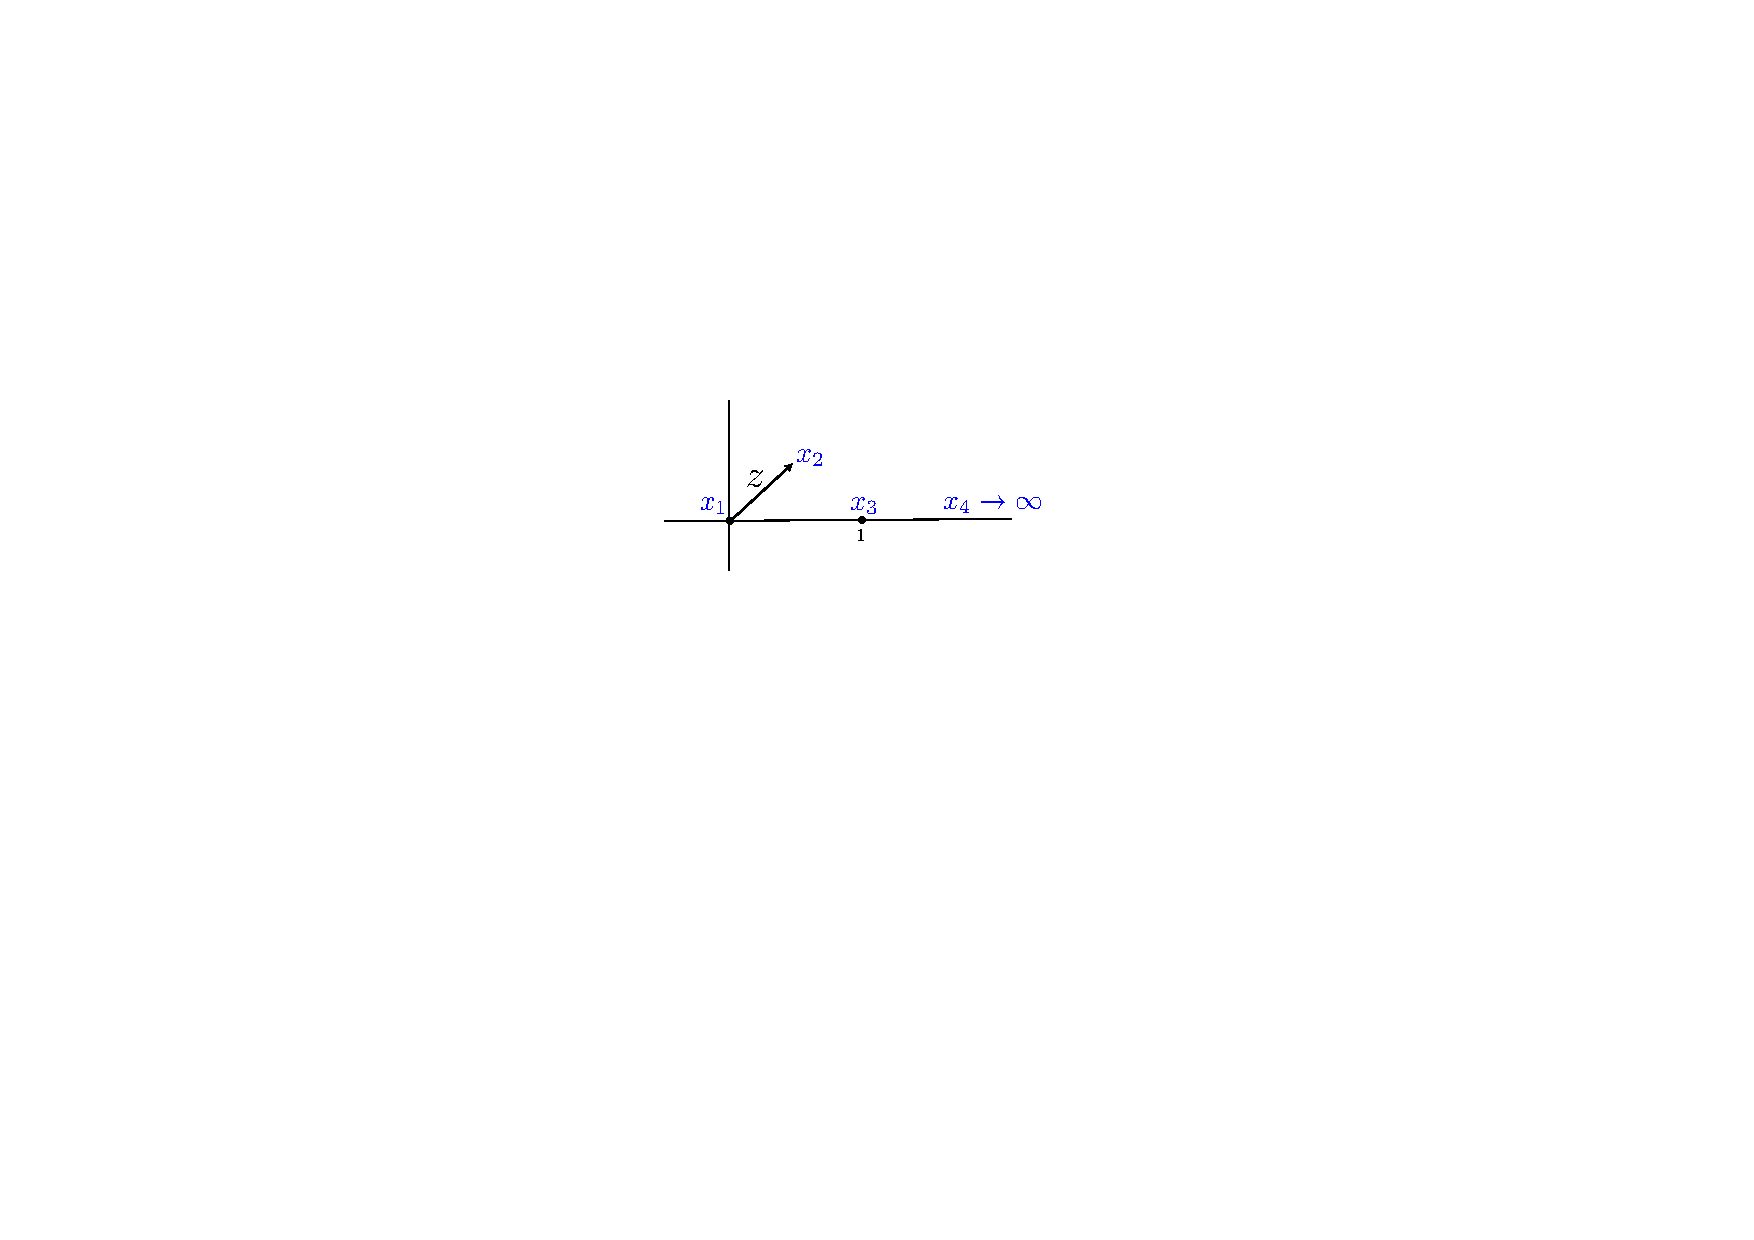
\includegraphics[width=0.4\textwidth]{fig-z}
\end{center}
\caption{\label{fig:zplane} Using conformal transformations in $d=2$ spacetime, any four points can be placed on a complex plane in the configuration shown above (from \cite{Hogervorst_2013}).}
\end{figure}
We have recovered the formula (\ref{eq:crossratio}) for cross-ratio in the previous section. Moreover, we can transform a line segment to a circle by conformal transformation, and one famous example is \textit{fractional linear transformations}. If we consider mapping line segment $x_{34}$ to a unit circle and line segment $x_{12}$ to a circle of radius $\rho$. And it turns out that the mapping is non-trivial than fractional linear transformation. If we consider placing $x_{i}$ in the following configuration
\begin{figure}[h]
\begin{center}
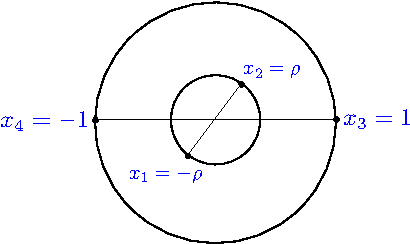
\includegraphics[width=0.55\textwidth]{fig-rho}
\end{center}
\caption{Any four points can be brought to the above configuration using conformal transformations. (from \cite{Hogervorst_2013}.)  \label{fig:rho}}
\end{figure}
The mapping is
\be
\label{eq:radialcoordinatedefinition}
w = \frac{z}{(1+\sqrt{1-z})^2},\qquad z = \frac{4w}{(1+w)^2}
\ee
Note that the non-trivial point of this mapping is that $x_1 = (0,0)$ in Fig.(\ref{fig:zplane}) is mapped to origin at first sight, but in fact, we should forget Fig.(\ref{fig:zplane}) and view (\ref{eq:radialcoordinatedefinition}) as a transformation of $z$. $u$ and $v$ are invariant under this transformation, so it is conformal:
\[
u = \frac{16w\bar{w}}{|w+1|^2|-w-1|^2} = z\bar z
\]
\[
v = \frac{|w-1|^2|-w+1|^2}{|-w-1|^2|w+1|^2} = (1-z)(1-\bar z)
\]
% (and similarly for $\bar\rho=r e^{-i\theta}$ and $\bar z$).
% \end{exercise}
Now we are ready to use this picture to derive the expansion of the conformal block, and now the radially ordered product of the 4-point correlation function is easily realized by demanding $|\rho|<1$ in Fig.(\ref{fig:rho}).

Since the spacetime points are now placed in a spherical symmetry way, Cylindrical quantization is a natural way to simplify the Euclidean space $\mathbb{R}^d$ to $(0, \infty) \times \mathbb{S}^{d-1}$ and promotes the radial distance as evolution "time" $\tau = -\ln(r)$. In cylindrical quantization, Fig(\ref{fig:rho}) corresponds to placing cylinder operators $\cO_{\text{cyl}}(\tau, \bn) = \exp(-\tau\Delta)\.\cO_{\text{rad}}(x=\exp(-\tau)\bn$ at diametrically opposite points $\pm \bn$ and $\pm \bn'$ on $\mathbb{S}^{d-1}$, with $\cos\th=\bn\.\bn'$, and with the pairs separated by time $\tau= -\ln r$ shown in Fig.(~\ref{fig:cylinderconfig}). If we denote $\bn'$ as $\cO_{1}$ and $\cO_{2}$ insertions, $\bn$ as $\cO_3$ and $\cO_4$, and we also define the state with normalization factor from (\ref{eq:newdefinitionofg})
\be
|\psi(\bn)\> &\equiv& \frac{4^{\De_\f}}{f_{\f\f\cO}}\phi_\mathrm{cyl}(0,\bn)\phi_\mathrm{cyl}(0,-\bn)|0\>,
\ee
where $4^{\De_\f}$ is from $x_{12}^{-2\De_\f} = (2|\rho|)^{-2\De_{\f}}$ then the conformal block is
\be
\label{eq:blockintermsofpsi}
 g_{\De}(u,v) &=& \<\psi(\bn)||\cO|e^{-\tau D}|\psi(\bn')\>,
\ee
where $\tau = -\ln(1-|\rho|)$.

\begin{figure}[h]
\begin{center}
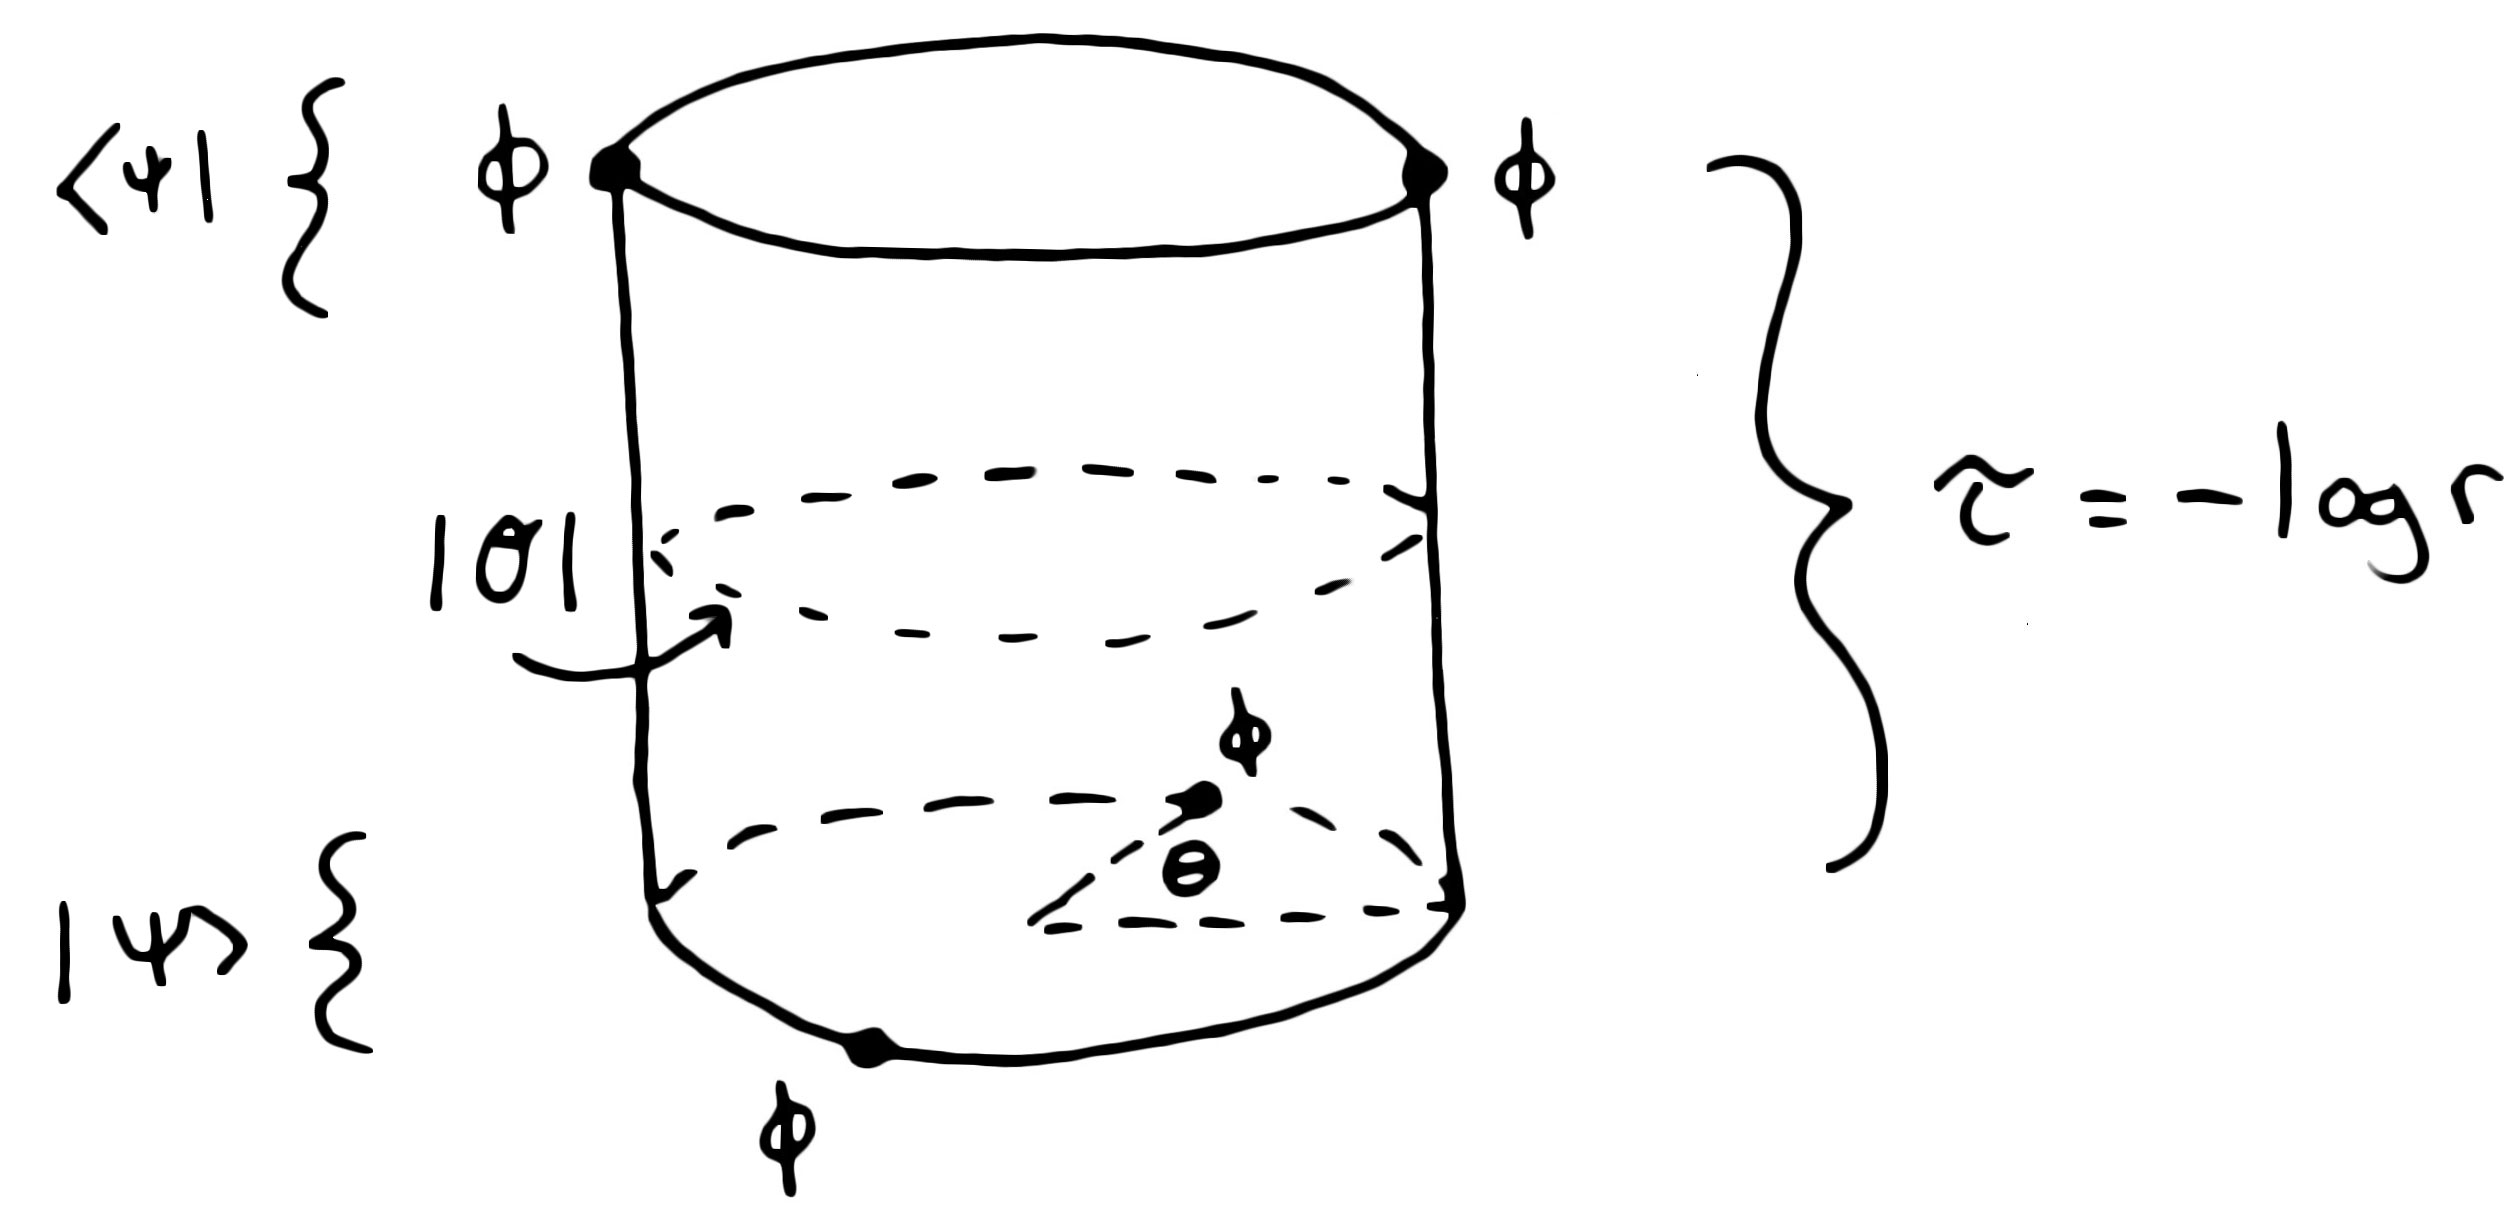
\includegraphics[width=0.75\textwidth]{cylinderconfig.jpg}
\end{center}
\caption{Configuration on the cylinder corresponding to (\ref{eq:blockintermsofpsi}).  \label{fig:cylinderconfig}}
\end{figure}

The eigenvalue of $D$ for a descendant $P^{\mu_1}\cdots P^{\mu_n}|\cO\>$ is $\De+n$ on the cylinder. 
Within the $n$-th level, the $\SO(d)$ spins of a spinless primary are caused by the momentum operator:
\be
\label{eq:rangeofjs}
j \in \{n,n-2,\dots\}.
\ee
Then we denote the set of descendant and primary states as $|n,j\>^{\mu_1\cdots\mu_j}$ with eigenvalue $\De+n$ and spin $j$. The projector $|\cO|$ as a summation of primaries and descendants, and (\ref{eq:blockintermsofpsi}) becomes
\be
r^{\De+n} \<\psi(\bn)|n,j\>^{\mu_1\cdots\mu_j}{}_{\mu_1\cdots\mu_j}\<n,j|\psi(\bn')\>,
\label{eq:definitespinandenergy}
\ee
where $r^{\De+n} = (1-|\rho|)^{\De+n}$ comes from the operator $\exp(-\tau\hat D)$.
By rotational invariance,
% \be
% \<\psi(\bn)|n,j\>^{\mu_1\cdots\mu_j} &\propto& \bn^{\mu_1}\cdots\bn^{\mu_j}-\mathrm{traces}.
% \ee
% Because $|\psi(\bn)\>=|\psi(-\bn)\>$, $j$ must be even (and thus $n$ is even).
Recall in the theory of hyperspherical harmonics, the Gegenbauer polynomial provides an orthogonal basis,
% \be
% C_j^{\frac{d-2}{2}}(\bn\cdot\bn') &\propto& (\bn^{\mu_1}\cdots\bn^{\mu_j}-\mathrm{traces})(\bn'_{\mu_1}\cdots\bn'_{\mu_j}-\mathrm{traces}),
% \ee
so (\ref{eq:definitespinandenergy}) can be expanded as
\be
r^{\De+n} \<\psi(\bn)|n,j\>^{\mu_1\cdots\mu_j}{}_{\mu_1\cdots\mu_j}\<n,j|\psi(\bn')\> &\propto& r^{\De+n}C_j^{\frac{d-2}{2}}(\cos\th),
\ee
where $\cos(\th) = \bn'\.\bn$

Summing over descendants, we find
\be
\label{eq:seriesexpansion}
g_{\De}(u,v) &=& \sum_{\substack{n=0,2,\dots \\ j}} B_{n,j}r^{\De+n}C_j^{\frac{d-2}{2}}(\cos\th),\label{eq:seriesforblock}
\ee
where $j$ goes over (\ref{eq:rangeofjs}) and $B_{n,j}$ are constant coefficients.  
Notice a few properties in \cite{simmonsduffin2016tasilecturesconformalbootstrap}:
\begin{itemize}
\item The leading term in the $r$ expansion comes from the primary state $|\cO\>$ with $n=0$ and $j=0$. This can be used as a boundary condition in the Casimir equation to determine the higher coefficients $B_{n,j}$.
\item The $B_{n,j}$ are positive in a unitary theory because they are given by norms of projections of $|\psi\>$ onto dilatation and spin eigenstates.
\item The $B_{n,j}$ are rational functions of $\De$.  This follows because the Casimir eigenvalue $\l_{\De}$ is polynomial in $\De$, or from the fact that the differential operators $C_a(x,\ptl)$ appearing in the OPE (\ref{eq:scalarscalarOPE}) have a series expansion in $x$ with rational coefficients. 
\end{itemize}

% \begin{exercise}
% \noindent\rule[0.5ex]{\linewidth}{1pt}
% Expand $g^{(2d)}_{\De}(u,v)$ and $g^{(4d)}_{\De}(u,v)$ to the first few orders in $r$, and check these properties.  Verify that some of the coefficients $B_{n,j}$ become negative when $\De$ violates the unitarity bound.
% \end{exercise}

% \begin{exercise}
(\ref{eq:seriesexpansion}) shows that spinless blocks are invariant under $x_1\leftrightarrow x_2$ or $x_3\leftrightarrow x_4$, where $r = 1-|\rho|$ is invariant and $\cos(\th) = \bn'\.\bn\rightarrow-\cos(\th)$, but $C^{\frac{d-2}{2}}_{j}(\cos\th)$ is symmetric function of $\cos\th$, and $u\rightarrow\frac u v,v\rightarrow\frac 1 v$,
\be
\label{eq:invariantunderonetwo}
g_{\De}(u,v) &=& g_{\De}\p{\frac{u}{v},\frac 1 v}
\ee
% \end{exercise}
% \noindent\rule[0.5ex]{\linewidth}{1pt}


\section{Conformal Bootstrap}
\subsection{OPE Associativity and Crossing Symmetry}

OPE determines $n$-point functions as sums of $(n-1)$-point functions,
\be
\label{eq:usingOPEtoreducecorrelator}
\<\cO_1(x_1)\cO_k(x_2)\cdots\cO_n(x_n)\> &=& \sum_k C_{12k}(x_{12},\ptl_2)\<\cO_2(x_2)\cdots\cO_n(x_n)\>,\nn\\
\ee
and finally in terms of $\De_i,f_{ijk}$, called "CFT data" as the differential operators $C_{ijk}(x,\ptl)$ are determined by conformal symmetry in terms of dimensions $\De_i$, spins, and 3-point correlation function coefficients $f_{ijk}$.

The bootstrap program uses consistent conditions to find out if a provided "CFT data" builds up a consistent CFT.

\begin{figure}[h]
\begin{center}
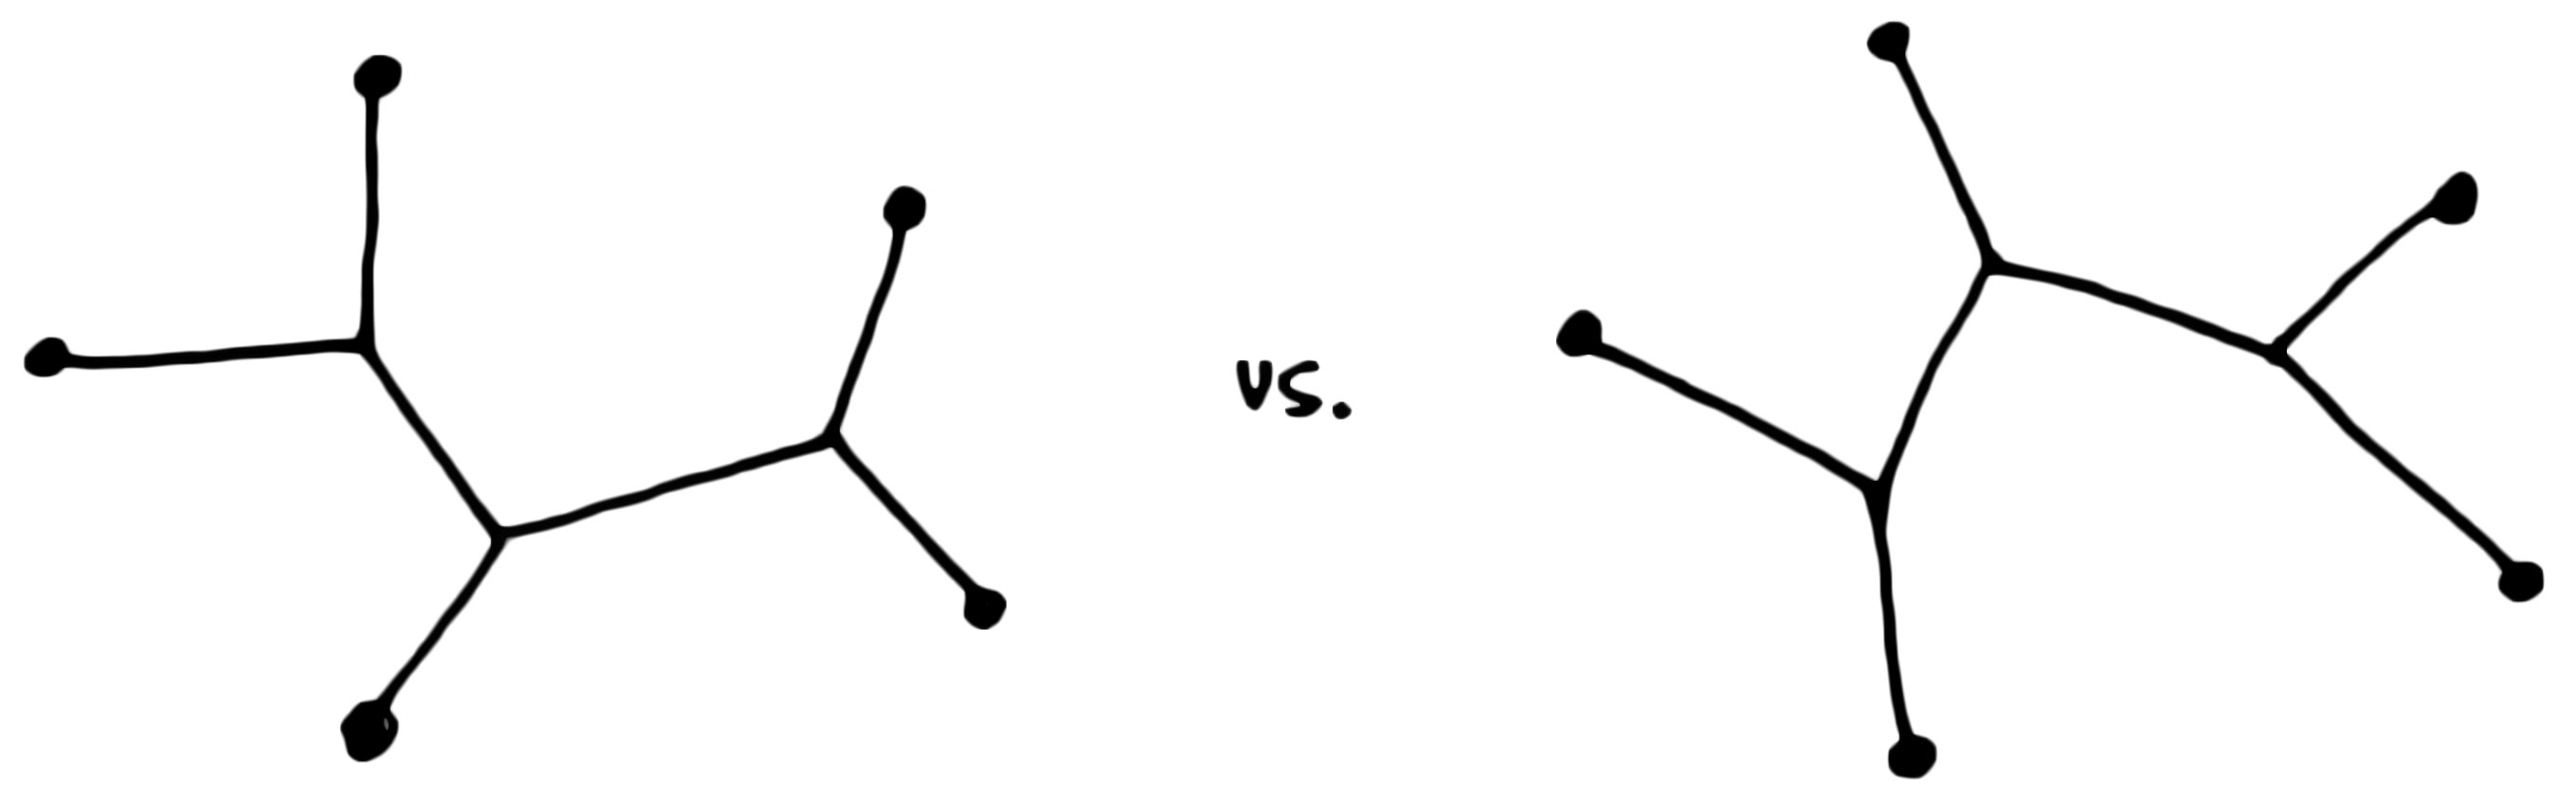
\includegraphics[width=0.75\textwidth]{opedifferentways.jpg}
\end{center}
\caption{Two different pairings of evaluating a five-point function using the OPE\@.  Dots represent operator insertions, and vertices represent the pairing order.\label{fig:opedifferentways}}
\end{figure}

Doing the OPE between different pairs of operators in different orders (see Fig~\ref{fig:opedifferentways}), we get different expressions for the same correlation function in terms of CFT data. There is no way to prevent them from being the same, it is the consistent conditions on the OPE.
\be
\contraction{}{
\frac 1 2\!\!\!\!\!
\cO_1\cO_2
}{}{\cO_3}
\contraction{}{\cO_1}{}{\cO_2}
\cO_1\cO_2\cO_3
&=&
\contraction{}{
\frac 1 2\!\!\!\!\!
\cO_1
}{}{
\contraction{}{\cO_2}{}{\cO_3}
\cO_2\cO_3
}
\contraction{\cO_1}{\cO_2}{}{\cO_3}
\cO_1\cO_2\cO_3,
\ee
or more explicitly,
\be
\label{eq:OPEassociativity}
C_{12i}(x_{12},\ptl_2)C_{i3j}(x_{23},\ptl_3)\cO_j(x_3) &=& C_{23i}(x_{23},\ptl_3)C_{1ij}(x_{13},\ptl_3)\cO_j(x_3).\nn\\
\ee
Consider additional $\cO_4(x_4)$ gives the so-called {\it crossing symmetry equation}

\be
\label{eq:graphicalcrossing}
\hspace{-0.4in}
\setlength{\unitlength}{.4in}
\begin{picture}(7,1.7)(0,0.2)
\linethickness{1pt}
\put(1.7,0.4){\line(1,2){0.3}}
\put(1.7,1.6){\line(1,-2){0.3}}
\put(2,1){\line(1,0){0.8}}
\put(2.8,1){\line(1,2){0.3}}
\put(2.8,1){\line(1,-2){0.3}}
\put(1.2,1){\makebox(0,0){$\mathlarger{\sum}_i^{\phantom\cO}$}}
\put(4,1){\makebox(0,0){$=$}}
\put(1.65,1.8){\makebox(0,0){\small $1$}}
\put(1.65,0.2){\makebox(0,0){\small $2$}}
\put(3.15,1.8){\makebox(0,0){\small $4$}}
\put(3.15,0.2){\makebox(0,0){\small $3$}}
\put(5.38,1.8){\makebox(0,0){\small $1$}}
\put(5.38,0.2){\makebox(0,0){\small $2$}}
\put(6.6,1.8){\makebox(0,0){\small $4$}}
\put(6.6,0.2){\makebox(0,0){\small $3$}}
\put(6.3,1){\makebox(0,0){\small $\cO_i$}}
\put(2.4,1.2){\makebox(0,0){\small $\cO_i$}}
\put(5,1){\makebox(0,0){$\mathlarger{\sum}_i^{\phantom\cO}$}}
\put(6,0.6){\line(0,1){0.8}}
\put(5.5,0.35){\line(2,1){0.5}}
\put(6,0.6){\line(2,-1){0.5}}
\put(6,1.38){\line(2,1){0.5}}
\put(5.5,1.65){\line(2,-1){0.5}}
\end{picture}.
\ee
The left-hand side is the conformal block expansion of $\<\cO_1\cO_2\cO_3\cO_4\>$ in the $12\leftrightarrow 34$ channel, while the right-hand side is the expansion in the $14\leftrightarrow 23$ channel. This is just an analog to describe conformal blocks as we do in scattering amplitudes.
% The crossing equation (\ref{eq:graphicalcrossing}) is a powerful but complicated constraint on the CFT data.  The rest of this course will be devoted to studying its implications for the simplest possible case: a four-point function of identical scalars $\<\f(x_1)\f(x_2)\f(x_3)\f(x_4)\>$.  

% \subsubsection{Additional Structures and Consistency Conditions}
\label{sec:additionalstructures}

% Before jumping in, let us reflect on the implications of exercise~\ref{ex:crossingexercise}:  A solution to the crossing equations~(\ref{eq:graphicalcrossing}) gives a completely nonperturbative definition of flat-space correlation functions of local operators, without the need for a Lagrangian.  This is most of the way towards a full theory. However, some structures associated with local QFTs are missing, and additional structures might bring new consistency conditions.

% Firstly, CFTs can admit extended objects like line operators, surface operators, boundaries, and interfaces. These objects have additional data associated with them, and it's possible to write down OPEs and crossing equations that relate this data to itself and the usual CFT data, see e.g. \cite{Liendo:2012hy,Gaiotto:2013nva}.  It is also interesting to consider correlation functions on manifolds not conformally equivalent to flat space. An example includes the theory at finite temperature (discussed in footnote~\ref{foot:finitetemperature}). This introduces more data, for example, the one-point functions of local and extended operators on nontrivial manifolds\footnote {It is known that this data is not determined by the local operator spectrum.  For example, pure Chern-Simons theory has no local operators at all but has interesting nonlocal observables that depend on the gauge group and level \cite{Witten:1988hf}.  Also, 4d conformal gauge theories admit different sets of line operators for the same set of local operators \cite{Aharony:2013hda}.} Other interesting constraints come from studying CFTs in Lorentzian signature. Examples include bounds from energy positivity \cite{Hofman:2008ar}, dispersion relations \cite{Komargodski:2011vj,Nachtmann:1973mr,Komargodski:2012ek,Komargodski:2016gci}, and causality \cite{Maldacena:2015waa,Hartman:2015lfa}.

% The full set of data and consistency conditions associated with a CFT is not known in general. However, we do have examples of constraints on local operators beyond the OPE and crossing equations. The most famous is modular invariance: the requirement that the partition function of a 2d CFT on the torus $T^2$ is invariant (or covariant) under large diffeomorphisms.  Imposing modular invariance is an additional step that must be performed after solving the crossing equations in 2d CFTs \cite{Moore:1988uz}.\footnote{2d is special because the space of states on a spatial slice $S^1\subset T^2$ is the same as the space of states in radial quantization, and thus modular invariance on $T^2$ directly constrains local operators.  This is not true in $d\geq 3$, so it is not clear how modular invariance on $T^d$ constrains local operators in that case.}

\subsection{Identical Scalar} 
Consider the 4-point correlation function of identical scalar field $\f$.
\begin{itemize}
\item We have the OPE
\be
\f(x_1)\f(x_2) &=& \sum_{\cO} f_{\f\f\cO} C(x_{12},\ptl_2) \cO(x_2),
\ee
where $\De$ is the dimension of $\cO$.

\item An orthonormal basis of operators $\cO$ are chosen as we did in (\ref{eq:canonicallynormalizedtwopt}).  Unitarity of the operator implies that the three-point coefficients $f_{\f\f\cO}$ are real.

\item Each spinless operator $\cO$ satisfies the unitarity bounds
\be
\label{eq:unitarityboundsummary}
\De &=& 0 \ \textrm{(unit operator), or}\nn\\
\De &=& \frac{d-2}{2}
\ee

\item The conformal block expansion for 4-point correlation functions, note the expansion is in $12\leftrightarrow34$ channel.
\be
\<\f(x_1)\f(x_2)\f(x_3)\f(x_4)\> &=& \frac{g(u,v)}{x_{12}^{2\De_\f}x_{34}^{2\De_\f}}\\
g(u,v) &=& \sum_\cO f_{\f\f\cO}^2 g_{\De}(u,v),
\ee
where $g_{\De}(u,v)$ are conformal blocks, and the cross ratios are
\be
u = z\bar z = \frac{x_{12}^2 x_{34}^2}{x_{13}^2 x_{24}^2},\qquad v=(1-z)(1-\bar z) =\frac{x_{23}^2 x_{14}^2}{x_{13}^2 x_{24}^2}.
\ee


\item Crossing symmetry is equivalent to the condition that the four-point function is invariant under the exchange $1\leftrightarrow 3$ or $2\leftrightarrow 4$ and $1\leftrightarrow2$ or $3\leftrightarrow4$,
\be
\label{eq:crossing1324}
g(u,v) &=& \p{\frac{u}{v}}^{\De_\f} g(v,u).
\ee
% Also (\ref{eq:invariantunderonetwo}) shows that invariance of the four-point function under $1\leftrightarrow 2$ or $3\leftrightarrow 4$.  
\be
\label{eq:crossing1234}
g(u,v) &=& g(\frac u v,\frac 1 v)
\ee
All other permutations can be generated from these.

\end{itemize}

% We know at least two operators present in the $\f\x\f$ OPE: the unit operator and the stress tensor.  Normalizing $\f$ so that $\<\f(x)\f(0)\>=x^{-2\De_\f}$, we have $f_{\f\f\mathbf{1}}=1$.  The stress tensor three-point coefficient is set by Ward identities to be $f_{\f\f T_{\mu\nu}}\propto \De_\f/\sqrt{C_T}$, where $C_T$ is the coefficient of the two-point function of the canonically normalized stress tensor (\ref{eq:twopointfunctionofspinL}).  The factor of $1/\sqrt{C_T}$ relative to (\ref{eq:stresstensorward}) comes from choosing the basis of operators $\cO$ to be orthonormal.
\subsection{An Infinite Number of Primaries}

Consider a limit $x_2\to x_1$, equivalent to $z\to 0$ with $z=\bar z$.

Recall that the blocks go like $g_{\De}(u,v) \sim u^{\De/2}(1+\cdots) \sim (z\bar z)^{\De/2}$ in this limit, so the left-hand side of (\ref{eq:crossing1324}) is dominated by the unit operator, which is the smallest dimension ($\De = 0$) operator in the OPE:
\be
\mathrm{LHS} &:& 1+\dots \qquad(z\to 0).
\ee

The crossing symmetry $u\leftrightarrow v$ corresponds to $(z,\bar z)\to (1-z,1-\bar z)$. 
In the limit $z\to 0$, each conformal block $g_{\De}((1-z)(1-\bar{z}),z\bar{z})\rightarrow\log z$.
% \begin{exercise}

% Check this for the explicit formulae (\ref{eq:explicitblock2d}) and (\ref{eq:explicitblock4d}).
% \end{exercise}
Thus, each term on the right-hand side goes like
\be
\label{eq:rhsterms}
\textrm{each term, RHS} &:& |z|^{2\De_\f}\ln |z| + \cdots \qquad(z\to 0).
\ee
As $z\to 0$, any finite sum of terms of the form (\ref{eq:rhsterms}) vanishes.  Thus, for a sum of operators on the right-hand side to reproduce that on the left-hand side, {\bf an infinite number of primary operators is needed}.
% \footnote{This doesn't contradict the textbook statement that rational 2d CFTs contain a finite number of primary operators.  In that context, ``primary" refers to primary operators concerning the Virasoro algebra.  Here, we are discussing primaries concerning the global conformal group, which is $\mathrm{SL}(2,\R)\x\mathrm{SL}(2,\R)$ in 2d.  A single Virasoro representation contains an infinite number of global conformal representations.}

% One can prove that as $z\to 0$, the sum on the right-hand side is dominated by operators of dimension $\Delta\sim 1/\sqrt z$ \cite{Pappadopulo:2012jk}.  
% In other words, the unit operator on the left-hand side maps to the large-$\De$ asymptotics of the sum over operators on the right-hand side.  
The general feature of the crossing equation (\ref{eq:graphicalcrossing}) is that it cannot be satisfied block-by-block.
% One can also show \cite{Pappadopulo:2012jk} that the conformal block expansion converges exponentially in $\De$ whenever $|\rho|\leq 1$, where $\rho$ is defined in (\ref{eq:radialcoordinatedefinition}).  In particular, this means that both sides of the crossing equation converge exponentially in a finite neighborhood of the point $z=\bar z=\frac 1 2$, which will play an important role in the next section.
Analyzing different limits of the crossing equation can give other consistent information about the distribution of $\De$ of primaries, which is called "CFT spectrum".  
% For example, the limit $z\to 0$ with $\bar z$ fixed gives information about operators with large spin \cite{Alday:2007mf,Fitzpatrick:2012yx,Komargodski:2012ek,Alday:2015ewa}.

% \subsection{Crossing Symmetry}
% \subsection{Spectrum of Primary Operator}
\section{Conclusion}

\section*{Appendix}
\subsection*{Derivation of Ward-Takahashi Identity for Stress Energy}
Recall the definition of stress-energy in QFT with a background metric $g$:
\begin{equation*}
    \langle T^{\mu\nu}(x)\mathcal{O}_1(x_1)\cdots\mathcal{O}_n(x_n)\rangle_g = \frac{2}{\sqrt{|g(x)|}}\frac{\delta}{\delta g_{\mu\nu}(x)}\langle\mathcal{O}_1(x_1)\cdots\mathcal{O}_n(x_n)\rangle_{g}
\end{equation*}
For simplicity, we consider only a single operator insertion $\mathcal{O}_1(x_1)$ in Eq(1.3):
\[
    \frac{2}{\sqrt{|g|}}\frac{\delta}{\delta g_{\mu\nu}}\langle\mathcal{O}_1(x_1)\rangle_g = \frac{2}{\sqrt{|g|}}\frac{\delta}{\delta g_{\mu\nu}}\int{\prod_{y}d\phi(y)\,}\mathcal{O}_1(x_1)e^{S[g,\phi]}
\]
\[
    = \frac{2}{\sqrt{|g|}}\int{\prod_{y}d\phi(y)\,}\left(\frac{\delta\mathcal{O}_1(x_1)}{\delta g_{\mu\nu}(x)}e^{-S[g,\phi]} - \mathcal{O}_1(x_1)e^{-S[g,\phi]}\frac{\delta S[g,\phi]}{\delta g_{\mu\nu}(x)}\right)
\]
Rewrite the operator $\mathcal{O}_1(x_1) = \int{d^4y\,} \sqrt{|g|}\delta^4(y-x_1)\mathcal{O}_1(y)/\sqrt{|g|}$:
\[
    \frac{\delta\sqrt{|g|}}{\delta g_{\mu\nu}} = \frac{\delta\exp(\frac{1}{2}\Tr\ln(g))}{\delta g_{\mu\nu}}
\]
\[
    =\frac{\sqrt{|g|}}{2}g^{\mu\nu}
\]

Then,
\[
    \frac{\delta\mathcal{O}_1(x_1)}{\delta g_{\mu\nu}(x)} = \int{d^4y\,\sqrt{|g|}}\delta^4(y-x_1)\mathcal{O}_1(y)\cdot(-\frac{1}{2\sqrt{|g|}}g^{\mu\nu})\delta^4(y-x)
\]
\[
    = -\frac{g^{\mu\nu}(x)}{2}\delta^4(x-x_1)\mathcal{O}_1(x_1)
\]
So the Ward-Takahashi identity of stress energy is Eq(1.3) under flat spacetime limit:
\[
     \partial_{\mu}\langle T^{\mu\nu}(x)\mathcal{O}_1(x_1)\rangle = -\partial^{\nu}\langle\delta^4(x-x_1)\mathcal{O}_1(x_1)\rangle
\]
\[
    = -\delta^4(x-x_1)\partial^{\nu}_{1}\langle\mathcal{O}_1(x_1)\rangle
\]
We've used integration by parts and disregarded the total derivative term, as the Ward-Takahashi identity has physical significance only when it is integrated over a spacetime volume, as in Eq(1.5).
\subsection*{Conformal Symmetry}
In sec 1.4, solutions of the conformal Killing equation give us special symmetry that keeps metric conformal, and in this section, we'll briefly go over some solutions \cite{DiFrancesco:1997nk}.
\subsubsection*{General Solutions}
Recall conformal Killing equation Eq.(1.10) and we can express $c(x)$ in terms of $\epsilon(x)$, it is possible to further settle down the form of conformal symmetry infinitesimally. Use a similar trick solving the relation of Christoffel symbols and metrics \cite{Carroll_2019}, applying an extra derivative on the conformal Killing equation, permuting the indices, and taking a linear combination \cite{DiFrancesco:1997nk}:
\[
    2\partial_{\mu}\partial_{\nu}\epsilon_{\rho} = \eta_{\mu\rho}\partial_{\nu}c+\eta_{\nu\rho}\partial_{\mu}c-\eta_{\mu\nu}\partial_{\rho}c
\]
Contracting the indices $\mu\text{ and }\nu$,
\[
    2\partial^2\epsilon_{\mu} = (2-d)\partial_{\mu}c
\]
Additionally, applying $\partial_{\nu}$ on this equation:
\[
    2\partial_{\nu}\partial^2\epsilon_{\mu} = (2-d)\partial_{\nu}\partial_{\mu}c
\]
compared with Eq.(1.10):
\[
    \partial_{\mu}\partial^2\epsilon_{\nu}+\partial_{\nu}\partial^2\epsilon_{\mu} = \eta_{\mu\nu}\partial^2c
\]
Now the L.H.S is $(2-d)\partial_{\nu}\partial_{\mu}c$, we have a differential equation of $c(x)$ along:
\[
    (d-1)\partial^2c(x) = 0
\]
We see that conformal symmetry is related to the dimension! In $d=1$, there is no restriction on $c(x)$, which means any smooth transformation would be conformal in $1D$ because the angle is meaningless in $1D$. Now if we consider $d\ge3$, then we must have:
\[
    \partial^2c(x) = 0
\]
thus function $c(x)$ is at most linear in coordinates:
\[
    c(x) = A + B_{\mu}x^{\mu} = \frac{2}{d}\partial\cdot\epsilon(x)
\]
In general, the infinitesimal parameter $\epsilon(x)$ is:
\[
    \epsilon_{\mu}(x) = a_{\mu} + b_{\mu\nu}x^{\nu}+c_{\mu\rho\nu}x^{\rho}x^{\nu}
\]
where $a,b,c$ are constant, and $c_{\mu\rho\nu} = c_{\mu\nu\rho}$. The constant term $a_{\mu}$ doesn't have any restriction and represents the infinitesimal translation in coordinates. Plug the solution back into the conformal Killing equation, the first-order part gives:
\[
    b_{\nu\mu}+b_{\mu\nu} = \frac{2}{d}b^{\rho}_{\,\,\,\rho}\eta_{\mu\nu}
\]
Therefore, the symmetric part of the coefficient of linear term is proportional to flat spacetime metric (as it should):
\[
    b_{\mu\nu} = \frac{1}{d}b^{\rho}_{\,\,\,\rho}\eta_{\mu\nu} + m_{\mu\nu}
\]
The symmetric part represents an infinitesimal scale transformation, and the anti-symmetric part is an infinitesimal rotation. Plug in the solution into a second-order differential equation, and the coefficient of the quadratic term can be expressed as:
\[
    c_{\mu\nu\rho} = \eta_{\mu\rho}\beta_{\nu}+\eta_{\nu\mu}\beta_{\rho}-\eta_{\nu\rho}\beta_{\mu}
\]
where $\beta_{\mu} = c^{\sigma}_{\,\,\,\sigma\mu}/d$, and the corresponding infinitesimal transformation is so-called \textbf{special conformal transformation} (SCT).
\subsubsection*{Dilatation Transformation}
We now focus on the dilatation transformation, characterized by:
\[
    \epsilon_{\mu}(x) = \frac{b^{\rho}_{\,\,\,\rho}}{d}x_{\mu}
\]

The corresponding conserved charge, derived from the stress-energy tensor, is given by:
\[
    Q_{\epsilon}(\Sigma) = -\int_{\Sigma} dS_{\mu}\, \frac{b^{\rho}_{\,\,\,\rho}}{d}x_{\nu}T^{\mu\nu}(x)
\]

This suggests a form for the generator that relates to the momentum operator, specifically:
\[
    d = x^{\mu}p_{\mu}
\]

Here, the momentum operator typically generates constant translations, but in this context, it acquires an explicit linear dependence on \( x \). Thus, in our formulation, the dilatation transformation is expected to generate:
\[
    x^{\mu} \rightarrow x'^{\mu} = x^{\mu} + \epsilon x^{\mu}
\]

However, this description is not fully rigorous, particularly when considering fields \( \phi(x) \) that possess a scaling dimension, as outlined in \cite{DiFrancesco:1997nk}. Despite this limitation, the relation between the conformal transformation (as defined in Eq. (1.9)) and the momentum operator (associated with spacetime translations) offers valuable intuition, even though a formal derivation would require additional considerations.

\subsubsection*{Special Conformal Transformations}

The generator of special conformal transformations is given by
\begin{equation*}
    k_{\mu} = 2x_{\mu}(x\cdot\partial) - x^2\partial_{\mu}
\end{equation*}

To interpret its physical meaning and the transformations it generates, we consider the inversion:
\begin{equation*}
    I: x^{\mu} \rightarrow x'^{\mu} = \frac{x^{\mu}}{x^2}
\end{equation*}

Following our approach in the last section, we assume the generator of special conformal transformations to be related to the momentum operator:
\[
    k^{\mu} = -I p^{\mu} I
\]
so that
\[
    -I p_{\mu} I = \frac{\partial}{\partial x'^{\mu}}
\]
\[
    = \frac{\partial x^{\nu}}{\partial x'^{\mu}} \frac{\partial}{\partial x^{\nu}}
\]
\[
    = -\left(x^2 \partial_{\mu} - 2x_{\mu}(x \cdot \partial)\right) = k_{\mu}
\]
where
\[
    \frac{\partial x'^{\mu}}{\partial x^{\nu}} = \frac{1}{x^4} \left(\delta^{\mu}_{\nu} x^2 - 2x^{\mu} x_{\nu}\right)
\]

Considering the finite transformation \( e^{a \cdot k} \) acting on \( x \), the special conformal transformation becomes manifest as a translation preceded and followed by an inversion:
\[
    x^{\mu} \rightarrow x_{\text{I}}^{\mu} = \frac{x^{\mu}}{x^2}
\]
\[
    x_{\text{I}}^{\mu} \rightarrow x_{\text{trans}}^{\mu} = \frac{x^{\mu}}{x^2} - a^{\mu}
\]
\[
    x_{\text{trans}}^{\mu} \rightarrow x_{\text{SCT}}^{\mu} = \frac{\frac{x^{\mu}}{x^2} - a^{\mu}}{\left(\frac{x^{\mu}}{x^2} - a^{\mu}\right)^2}
\]
\[
    = \frac{x^{\mu} - a^{\mu} x^2}{x^2 - 2(a \cdot x) + a^2}
\]

If \( a^{\mu} \) is taken to be infinitesimal, this recovers the solution to the conformal Killing equation discussed in the previous section. Notably, the special conformal transformation (SCT) can be viewed as a transformation that shifts infinity while leaving the origin fixed.

\bibliographystyle{plain}
\bibliography{ref}
\end{document}